\documentclass[1p]{elsarticle_modified}
%\bibliographystyle{elsarticle-num}

%\usepackage[colorlinks]{hyperref}
%\usepackage{abbrmath_seonhwa} %\Abb, \Ascr, \Acal ,\Abf, \Afrak
\usepackage{amsfonts}
\usepackage{amssymb}
\usepackage{amsmath}
\usepackage{amsthm}
\usepackage{scalefnt}
\usepackage{amsbsy}
\usepackage{kotex}
\usepackage{caption}
\usepackage{subfig}
\usepackage{color}
\usepackage{graphicx}
\usepackage{xcolor} %% white, black, red, green, blue, cyan, magenta, yellow
\usepackage{float}
\usepackage{setspace}
\usepackage{hyperref}

\usepackage{tikz}
\usetikzlibrary{arrows}

\usepackage{multirow}
\usepackage{array} % fixed length table
\usepackage{hhline}

%%%%%%%%%%%%%%%%%%%%%
\makeatletter
\renewcommand*\env@matrix[1][\arraystretch]{%
	\edef\arraystretch{#1}%
	\hskip -\arraycolsep
	\let\@ifnextchar\new@ifnextchar
	\array{*\c@MaxMatrixCols c}}
\makeatother %https://tex.stackexchange.com/questions/14071/how-can-i-increase-the-line-spacing-in-a-matrix
%%%%%%%%%%%%%%%

\usepackage[normalem]{ulem}

\newcommand{\msout}[1]{\ifmmode\text{\sout{\ensuremath{#1}}}\else\sout{#1}\fi}
%SOURCE: \msout is \stkout macro in https://tex.stackexchange.com/questions/20609/strikeout-in-math-mode

\newcommand{\cancel}[1]{
	\ifmmode
	{\color{red}\msout{#1}}
	\else
	{\color{red}\sout{#1}}
	\fi
}

\newcommand{\add}[1]{
	{\color{blue}\uwave{#1}}
}

\newcommand{\replace}[2]{
	\ifmmode
	{\color{red}\msout{#1}}{\color{blue}\uwave{#2}}
	\else
	{\color{red}\sout{#1}}{\color{blue}\uwave{#2}}
	\fi
}

\newcommand{\Sol}{\mathcal{S}} %segment
\newcommand{\D}{D} %diagram
\newcommand{\A}{\mathcal{A}} %arc


%%%%%%%%%%%%%%%%%%%%%%%%%%%%%5 test

\def\sl{\operatorname{\textup{SL}}(2,\Cbb)}
\def\psl{\operatorname{\textup{PSL}}(2,\Cbb)}
\def\quan{\mkern 1mu \triangleright \mkern 1mu}

\theoremstyle{definition}
\newtheorem{thm}{Theorem}[section]
\newtheorem{prop}[thm]{Proposition}
\newtheorem{lem}[thm]{Lemma}
\newtheorem{ques}[thm]{Question}
\newtheorem{cor}[thm]{Corollary}
\newtheorem{defn}[thm]{Definition}
\newtheorem{exam}[thm]{Example}
\newtheorem{rmk}[thm]{Remark}
\newtheorem{alg}[thm]{Algorithm}

\newcommand{\I}{\sqrt{-1}}
\begin{document}

%\begin{frontmatter}
%
%\title{Boundary parabolic representations of knots up to 8 crossings}
%
%%% Group authors per affiliation:
%\author{Yunhi Cho} 
%\address{Department of Mathematics, University of Seoul, Seoul, Korea}
%\ead{yhcho@uos.ac.kr}
%
%
%\author{Seonhwa Kim} %\fnref{s_kim}}
%\address{Center for Geometry and Physics, Institute for Basic Science, Pohang, 37673, Korea}
%\ead{ryeona17@ibs.re.kr}
%
%\author{Hyuk Kim}
%\address{Department of Mathematical Sciences, Seoul National University, Seoul 08826, Korea}
%\ead{hyukkim@snu.ac.kr}
%
%\author{Seokbeom Yoon}
%\address{Department of Mathematical Sciences, Seoul National University, Seoul, 08826,  Korea}
%\ead{sbyoon15@snu.ac.kr}
%
%\begin{abstract}
%We find all boundary parabolic representation of knots up to 8 crossings.
%
%\end{abstract}
%\begin{keyword}
%    \MSC[2010] 57M25 
%\end{keyword}
%
%\end{frontmatter}

%\linenumbers
%\tableofcontents
%
\newcommand\colored[1]{\textcolor{white}{\rule[-0.35ex]{0.8em}{1.4ex}}\kern-0.8em\color{red} #1}%
%\newcommand\colored[1]{\textcolor{white}{ #1}\kern-2.17ex	\textcolor{white}{ #1}\kern-1.81ex	\textcolor{white}{ #1}\kern-2.15ex\color{red}#1	}

{\Large $\underline{12a_{0697}~(K12a_{0697})}$}

\setlength{\tabcolsep}{10pt}
\renewcommand{\arraystretch}{1.6}
\vspace{1cm}\begin{tabular}{m{100pt}>{\centering\arraybackslash}m{274pt}}
\multirow{5}{120pt}{
	\centering
	\includegraphics[width=112pt]{../../../GIT/diagram.site/Diagrams/png/1498_12a_0697.png}\\
\ \ \ A knot diagram\footnotemark}&
\allowdisplaybreaks
\textbf{Linearized knot diagam} \\
\cline{2-2}
 &
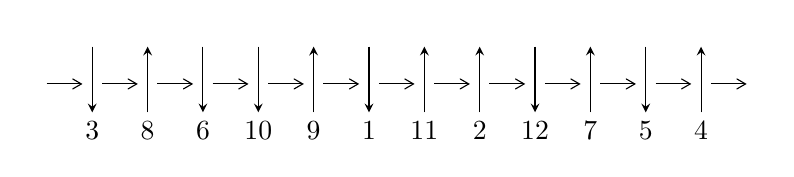
\begin{tikzpicture}[x=20pt, y=17pt]
	% nodes
	\node (C0) at (0, 0) {};
	\node (C1) at (1, 0) {};
	\node (C1U) at (1, +1) {};
	\node (C1D) at (1, -1) {3};

	\node (C2) at (2, 0) {};
	\node (C2U) at (2, +1) {};
	\node (C2D) at (2, -1) {8};

	\node (C3) at (3, 0) {};
	\node (C3U) at (3, +1) {};
	\node (C3D) at (3, -1) {6};

	\node (C4) at (4, 0) {};
	\node (C4U) at (4, +1) {};
	\node (C4D) at (4, -1) {10};

	\node (C5) at (5, 0) {};
	\node (C5U) at (5, +1) {};
	\node (C5D) at (5, -1) {9};

	\node (C6) at (6, 0) {};
	\node (C6U) at (6, +1) {};
	\node (C6D) at (6, -1) {1};

	\node (C7) at (7, 0) {};
	\node (C7U) at (7, +1) {};
	\node (C7D) at (7, -1) {11};

	\node (C8) at (8, 0) {};
	\node (C8U) at (8, +1) {};
	\node (C8D) at (8, -1) {2};

	\node (C9) at (9, 0) {};
	\node (C9U) at (9, +1) {};
	\node (C9D) at (9, -1) {12};

	\node (C10) at (10, 0) {};
	\node (C10U) at (10, +1) {};
	\node (C10D) at (10, -1) {7};

	\node (C11) at (11, 0) {};
	\node (C11U) at (11, +1) {};
	\node (C11D) at (11, -1) {5};

	\node (C12) at (12, 0) {};
	\node (C12U) at (12, +1) {};
	\node (C12D) at (12, -1) {4};
	\node (C13) at (13, 0) {};

	% arrows
	\draw[->,>={angle 60}]
	(C0) edge (C1) (C1) edge (C2) (C2) edge (C3) (C3) edge (C4) (C4) edge (C5) (C5) edge (C6) (C6) edge (C7) (C7) edge (C8) (C8) edge (C9) (C9) edge (C10) (C10) edge (C11) (C11) edge (C12) (C12) edge (C13) ;	\draw[->,>=stealth]
	(C1U) edge (C1D) (C2D) edge (C2U) (C3U) edge (C3D) (C4U) edge (C4D) (C5D) edge (C5U) (C6U) edge (C6D) (C7D) edge (C7U) (C8D) edge (C8U) (C9U) edge (C9D) (C10D) edge (C10U) (C11U) edge (C11D) (C12D) edge (C12U) ;
	\end{tikzpicture} \\
\hhline{~~} \\& 
\textbf{Solving Sequence} \\ \cline{2-2} 
 &
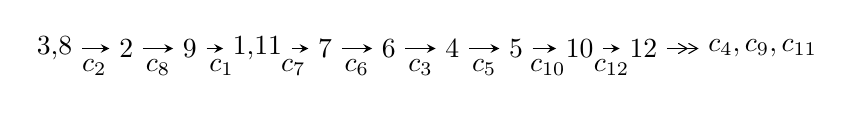
\begin{tikzpicture}[x=23pt, y=7pt]
	% node
	\node (A0) at (-1/8, 0) {3,8};
	\node (A1) at (1, 0) {2};
	\node (A2) at (2, 0) {9};
	\node (A3) at (49/16, 0) {1,11};
	\node (A4) at (33/8, 0) {7};
	\node (A5) at (41/8, 0) {6};
	\node (A6) at (49/8, 0) {4};
	\node (A7) at (57/8, 0) {5};
	\node (A8) at (65/8, 0) {10};
	\node (A9) at (73/8, 0) {12};
	\node (C1) at (1/2, -1) {$c_{2}$};
	\node (C2) at (3/2, -1) {$c_{8}$};
	\node (C3) at (5/2, -1) {$c_{1}$};
	\node (C4) at (29/8, -1) {$c_{7}$};
	\node (C5) at (37/8, -1) {$c_{6}$};
	\node (C6) at (45/8, -1) {$c_{3}$};
	\node (C7) at (53/8, -1) {$c_{5}$};
	\node (C8) at (61/8, -1) {$c_{10}$};
	\node (C9) at (69/8, -1) {$c_{12}$};
	\node (A10) at (11, 0) {$c_{4},c_{9},c_{11}$};

	% edge
	\draw[->,>=stealth]	
	(A0) edge (A1) (A1) edge (A2) (A2) edge (A3) (A3) edge (A4) (A4) edge (A5) (A5) edge (A6) (A6) edge (A7) (A7) edge (A8) (A8) edge (A9) ;
	\draw[->>,>={angle 60}]	
	(A9) edge (A10);
\end{tikzpicture} \\ 

\end{tabular} \\

\footnotetext{
The image of knot diagram is generated by the software ``\textbf{Draw programme}" developed by Andrew Bartholomew(\url{http://www.layer8.co.uk/maths/draw/index.htm\#Running-draw}), where we modified some parts for our purpose(\url{https://github.com/CATsTAILs/LinksPainter}).
}\phantom \\ \newline 
\centering \textbf{Ideals for irreducible components\footnotemark of $X_{\text{par}}$} 
 
\begin{align*}
I^u_{1}&=\langle 
-1.38429\times10^{798} u^{193}+3.87152\times10^{798} u^{192}+\cdots+2.19950\times10^{798} b-4.90381\times10^{800},\\
\phantom{I^u_{1}}&\phantom{= \langle  }-8.75612\times10^{800} u^{193}+3.14690\times10^{801} u^{192}+\cdots+2.64159\times10^{801} a+2.08172\times10^{803},\\
\phantom{I^u_{1}}&\phantom{= \langle  }u^{194}-4 u^{193}+\cdots-2190 u+1201\rangle \\
I^u_{2}&=\langle 
1.01475\times10^{22} u^{43}-2.00856\times10^{22} u^{42}+\cdots+3.01682\times10^{21} b-9.17444\times10^{21},\\
\phantom{I^u_{2}}&\phantom{= \langle  }-6.80246\times10^{21} u^{43}+1.04596\times10^{22} u^{42}+\cdots+3.01682\times10^{21} a-1.46523\times10^{22},\;u^{44}- u^{43}+\cdots-5 u+1\rangle \\
\\
\end{align*}
\raggedright * 2 irreducible components of $\dim_{\mathbb{C}}=0$, with total 238 representations.\\
\footnotetext{All coefficients of polynomials are rational numbers. But the coefficients are sometimes approximated in decimal forms when there is not enough margin.}
\newpage
\renewcommand{\arraystretch}{1}
\centering \section*{I. $I^u_{1}= \langle -1.38\times10^{798} u^{193}+3.87\times10^{798} u^{192}+\cdots+2.20\times10^{798} b-4.90\times10^{800},\;-8.76\times10^{800} u^{193}+3.15\times10^{801} u^{192}+\cdots+2.64\times10^{801} a+2.08\times10^{803},\;u^{194}-4 u^{193}+\cdots-2190 u+1201 \rangle$}
\flushleft \textbf{(i) Arc colorings}\\
\begin{tabular}{m{7pt} m{180pt} m{7pt} m{180pt} }
\flushright $a_{3}=$&$\begin{pmatrix}1\\0\end{pmatrix}$ \\
\flushright $a_{8}=$&$\begin{pmatrix}0\\u\end{pmatrix}$ \\
\flushright $a_{2}=$&$\begin{pmatrix}1\\u^2\end{pmatrix}$ \\
\flushright $a_{9}=$&$\begin{pmatrix}u\\u^3+u\end{pmatrix}$ \\
\flushright $a_{1}=$&$\begin{pmatrix}u^2+1\\u^2\end{pmatrix}$ \\
\flushright $a_{11}=$&$\begin{pmatrix}0.331471 u^{193}-1.19129 u^{192}+\cdots+396.308 u-78.8056\\0.629367 u^{193}-1.76019 u^{192}+\cdots+443.354 u+222.952\end{pmatrix}$ \\
\flushright $a_{7}=$&$\begin{pmatrix}0.230235 u^{193}-0.229303 u^{192}+\cdots-256.608 u+636.997\\2.04507 u^{193}-7.51758 u^{192}+\cdots+3825.85 u-1438.51\end{pmatrix}$ \\
\flushright $a_{6}=$&$\begin{pmatrix}-0.584614 u^{193}+2.07784 u^{192}+\cdots-968.110 u+357.563\\1.02690 u^{193}-3.46100 u^{192}+\cdots+1531.49 u-314.193\end{pmatrix}$ \\
\flushright $a_{4}=$&$\begin{pmatrix}0.316417 u^{193}-0.526957 u^{192}+\cdots-603.289 u+840.527\\0.639153 u^{193}-1.96569 u^{192}+\cdots+543.699 u+4.23901\end{pmatrix}$ \\
\flushright $a_{5}=$&$\begin{pmatrix}0.341625 u^{193}-0.495401 u^{192}+\cdots-230.907 u+752.488\\2.03737 u^{193}-7.36267 u^{192}+\cdots+3634.73 u-1278.45\end{pmatrix}$ \\
\flushright $a_{10}=$&$\begin{pmatrix}0.899157 u^{193}-3.33150 u^{192}+\cdots+1895.23 u-716.726\\0.423782 u^{193}-2.40417 u^{192}+\cdots+1856.81 u-1315.96\end{pmatrix}$ \\
\flushright $a_{12}=$&$\begin{pmatrix}0.636085 u^{193}-2.44361 u^{192}+\cdots+1676.72 u-722.342\\0.241514 u^{193}-1.40839 u^{192}+\cdots+1124.19 u-730.575\end{pmatrix}$\\&\end{tabular}
\flushleft \textbf{(ii) Obstruction class $= -1$}\\~\\
\flushleft \textbf{(iii) Cusp Shapes $= -2.45492 u^{193}+7.04924 u^{192}+\cdots-2454.11 u-495.711$}\\~\\
\newpage\renewcommand{\arraystretch}{1}
\flushleft \textbf{(iv) u-Polynomials at the component}\newline \\
\begin{tabular}{m{50pt}|m{274pt}}
Crossings & \hspace{64pt}u-Polynomials at each crossing \\
\hline $$\begin{aligned}c_{1}\end{aligned}$$&$\begin{aligned}
&u^{194}+76 u^{193}+\cdots+17206220 u+1442401
\end{aligned}$\\
\hline $$\begin{aligned}c_{2},c_{8}\end{aligned}$$&$\begin{aligned}
&u^{194}+4 u^{193}+\cdots+2190 u+1201
\end{aligned}$\\
\hline $$\begin{aligned}c_{3}\end{aligned}$$&$\begin{aligned}
&16(16 u^{194}+316 u^{193}+\cdots-5 u+1)
\end{aligned}$\\
\hline $$\begin{aligned}c_{4}\end{aligned}$$&$\begin{aligned}
&4(4 u^{194}+6 u^{193}+\cdots-180 u+5)
\end{aligned}$\\
\hline $$\begin{aligned}c_{5}\end{aligned}$$&$\begin{aligned}
&u^{194}-4 u^{193}+\cdots+223613010 u+9397652
\end{aligned}$\\
\hline $$\begin{aligned}c_{6}\end{aligned}$$&$\begin{aligned}
&u^{194}+4 u^{192}+\cdots+535380 u+59536
\end{aligned}$\\
\hline $$\begin{aligned}c_{7},c_{10}\end{aligned}$$&$\begin{aligned}
&4(4 u^{194}+10 u^{193}+\cdots-2 u+1)
\end{aligned}$\\
\hline $$\begin{aligned}c_{9}\end{aligned}$$&$\begin{aligned}
&u^{194}-19 u^{193}+\cdots-8 u+1
\end{aligned}$\\
\hline $$\begin{aligned}c_{11}\end{aligned}$$&$\begin{aligned}
&4(4 u^{194}+30 u^{193}+\cdots-60 u+1)
\end{aligned}$\\
\hline $$\begin{aligned}c_{12}\end{aligned}$$&$\begin{aligned}
&u^{194}+9 u^{193}+\cdots+38561386 u+5467612
\end{aligned}$\\
\hline
\end{tabular}\\~\\
\newpage\renewcommand{\arraystretch}{1}
\flushleft \textbf{(v) Riley Polynomials at the component}\newline \\
\begin{tabular}{m{50pt}|m{274pt}}
Crossings & \hspace{64pt}Riley Polynomials at each crossing \\
\hline $$\begin{aligned}c_{1}\end{aligned}$$&$\begin{aligned}
&y^{194}+20 y^{193}+\cdots-483570365808132 y+2080520644801
\end{aligned}$\\
\hline $$\begin{aligned}c_{2},c_{8}\end{aligned}$$&$\begin{aligned}
&y^{194}+76 y^{193}+\cdots+17206220 y+1442401
\end{aligned}$\\
\hline $$\begin{aligned}c_{3}\end{aligned}$$&$\begin{aligned}
&256(256 y^{194}-7920 y^{193}+\cdots-805 y+1)
\end{aligned}$\\
\hline $$\begin{aligned}c_{4}\end{aligned}$$&$\begin{aligned}
&16(16 y^{194}-476 y^{193}+\cdots+350 y+25)
\end{aligned}$\\
\hline $$\begin{aligned}c_{5}\end{aligned}$$&$\begin{aligned}
&y^{194}+56 y^{193}+\cdots-15147856641788764 y+88315863113104
\end{aligned}$\\
\hline $$\begin{aligned}c_{6}\end{aligned}$$&$\begin{aligned}
&y^{194}+8 y^{193}+\cdots-1377094192048 y+3544535296
\end{aligned}$\\
\hline $$\begin{aligned}c_{7},c_{10}\end{aligned}$$&$\begin{aligned}
&16(16 y^{194}-1740 y^{193}+\cdots-54 y+1)
\end{aligned}$\\
\hline $$\begin{aligned}c_{9}\end{aligned}$$&$\begin{aligned}
&y^{194}-27 y^{193}+\cdots+176 y+1
\end{aligned}$\\
\hline $$\begin{aligned}c_{11}\end{aligned}$$&$\begin{aligned}
&16(16 y^{194}-188 y^{193}+\cdots-218 y+1)
\end{aligned}$\\
\hline $$\begin{aligned}c_{12}\end{aligned}$$&$\begin{aligned}
&y^{194}+27 y^{193}+\cdots+83542449688324 y+29894780982544
\end{aligned}$\\
\hline
\end{tabular}\\~\\
\newpage\flushleft \textbf{(vi) Complex Volumes and Cusp Shapes}
$$\begin{array}{c|c|c}  
\text{Solutions to }I^u_{1}& \I (\text{vol} + \sqrt{-1}CS) & \text{Cusp shape}\\
 \hline 
\begin{aligned}
u &= -0.352856 + 0.935267 I \\
a &= -0.142936 + 1.156860 I \\
b &= -1.019070 - 0.047088 I\end{aligned}
 & -2.04059 + 1.29524 I & \phantom{-0.000000 } 0 \\ \hline\begin{aligned}
u &= -0.352856 - 0.935267 I \\
a &= -0.142936 - 1.156860 I \\
b &= -1.019070 + 0.047088 I\end{aligned}
 & -2.04059 - 1.29524 I & \phantom{-0.000000 } 0 \\ \hline\begin{aligned}
u &= -0.858241 + 0.500645 I \\
a &= -0.871810 + 0.893397 I \\
b &= -0.367726 + 0.658728 I\end{aligned}
 & -1.12610 + 9.17491 I & \phantom{-0.000000 } 0 \\ \hline\begin{aligned}
u &= -0.858241 - 0.500645 I \\
a &= -0.871810 - 0.893397 I \\
b &= -0.367726 - 0.658728 I\end{aligned}
 & -1.12610 - 9.17491 I & \phantom{-0.000000 } 0 \\ \hline\begin{aligned}
u &= \phantom{-}0.171791 + 0.977728 I \\
a &= -0.081012 - 0.481370 I \\
b &= -1.106520 - 0.429809 I\end{aligned}
 & -2.44322 - 1.19674 I & \phantom{-0.000000 } 0 \\ \hline\begin{aligned}
u &= \phantom{-}0.171791 - 0.977728 I \\
a &= -0.081012 + 0.481370 I \\
b &= -1.106520 + 0.429809 I\end{aligned}
 & -2.44322 + 1.19674 I & \phantom{-0.000000 } 0 \\ \hline\begin{aligned}
u &= \phantom{-}0.461501 + 0.900448 I \\
a &= \phantom{-}0.409589 - 0.627996 I \\
b &= \phantom{-}4.07565 + 2.62467 I\end{aligned}
 & -3.87773 + 6.12031 I & \phantom{-0.000000 } 0 \\ \hline\begin{aligned}
u &= \phantom{-}0.461501 - 0.900448 I \\
a &= \phantom{-}0.409589 + 0.627996 I \\
b &= \phantom{-}4.07565 - 2.62467 I\end{aligned}
 & -3.87773 - 6.12031 I & \phantom{-0.000000 } 0 \\ \hline\begin{aligned}
u &= -0.466956 + 0.870291 I \\
a &= \phantom{-}1.03500 + 1.16180 I \\
b &= \phantom{-}2.20505 - 1.18125 I\end{aligned}
 & -1.16359 - 1.62170 I & \phantom{-0.000000 } 0 \\ \hline\begin{aligned}
u &= -0.466956 - 0.870291 I \\
a &= \phantom{-}1.03500 - 1.16180 I \\
b &= \phantom{-}2.20505 + 1.18125 I\end{aligned}
 & -1.16359 + 1.62170 I & \phantom{-0.000000 } 0\\
 \hline 
 \end{array}$$\newpage$$\begin{array}{c|c|c}  
\text{Solutions to }I^u_{1}& \I (\text{vol} + \sqrt{-1}CS) & \text{Cusp shape}\\
 \hline 
\begin{aligned}
u &= \phantom{-}0.444555 + 0.881941 I \\
a &= \phantom{-}1.043030 + 0.571776 I \\
b &= \phantom{-}0.02131 + 1.64378 I\end{aligned}
 & -4.76293 + 1.82373 I & \phantom{-0.000000 } 0 \\ \hline\begin{aligned}
u &= \phantom{-}0.444555 - 0.881941 I \\
a &= \phantom{-}1.043030 - 0.571776 I \\
b &= \phantom{-}0.02131 - 1.64378 I\end{aligned}
 & -4.76293 - 1.82373 I & \phantom{-0.000000 } 0 \\ \hline\begin{aligned}
u &= -0.473853 + 0.899736 I \\
a &= -0.79929 - 1.33512 I \\
b &= -2.15545 + 0.63487 I\end{aligned}
 & -1.25921 - 2.17281 I & \phantom{-0.000000 } 0 \\ \hline\begin{aligned}
u &= -0.473853 - 0.899736 I \\
a &= -0.79929 + 1.33512 I \\
b &= -2.15545 - 0.63487 I\end{aligned}
 & -1.25921 + 2.17281 I & \phantom{-0.000000 } 0 \\ \hline\begin{aligned}
u &= \phantom{-}0.270488 + 0.939040 I \\
a &= \phantom{-}0.502282 + 1.260000 I \\
b &= -0.078034 + 0.758939 I\end{aligned}
 & -1.60615 - 6.44241 I & \phantom{-0.000000 } 0 \\ \hline\begin{aligned}
u &= \phantom{-}0.270488 - 0.939040 I \\
a &= \phantom{-}0.502282 - 1.260000 I \\
b &= -0.078034 - 0.758939 I\end{aligned}
 & -1.60615 + 6.44241 I & \phantom{-0.000000 } 0 \\ \hline\begin{aligned}
u &= \phantom{-}0.452051 + 0.858999 I \\
a &= -0.484321 + 0.613005 I \\
b &= -4.38482 - 2.55892 I\end{aligned}
 & -3.72430 - 2.38599 I & \phantom{-0.000000 } 0 \\ \hline\begin{aligned}
u &= \phantom{-}0.452051 - 0.858999 I \\
a &= -0.484321 - 0.613005 I \\
b &= -4.38482 + 2.55892 I\end{aligned}
 & -3.72430 + 2.38599 I & \phantom{-0.000000 } 0 \\ \hline\begin{aligned}
u &= -0.507795 + 0.897267 I \\
a &= -0.081761 + 1.334530 I \\
b &= \phantom{-}0.456448 - 0.037680 I\end{aligned}
 & -0.84339 - 2.73028 I & \phantom{-0.000000 } 0 \\ \hline\begin{aligned}
u &= -0.507795 - 0.897267 I \\
a &= -0.081761 - 1.334530 I \\
b &= \phantom{-}0.456448 + 0.037680 I\end{aligned}
 & -0.84339 + 2.73028 I & \phantom{-0.000000 } 0\\
 \hline 
 \end{array}$$\newpage$$\begin{array}{c|c|c}  
\text{Solutions to }I^u_{1}& \I (\text{vol} + \sqrt{-1}CS) & \text{Cusp shape}\\
 \hline 
\begin{aligned}
u &= -0.527035 + 0.807287 I \\
a &= \phantom{-}1.27885 - 1.51703 I \\
b &= -0.24618 - 1.44845 I\end{aligned}
 & -1.80592 - 2.20740 I & \phantom{-0.000000 } 0 \\ \hline\begin{aligned}
u &= -0.527035 - 0.807287 I \\
a &= \phantom{-}1.27885 + 1.51703 I \\
b &= -0.24618 + 1.44845 I\end{aligned}
 & -1.80592 + 2.20740 I & \phantom{-0.000000 } 0 \\ \hline\begin{aligned}
u &= -0.545883 + 0.792695 I \\
a &= \phantom{-}0.333347 + 1.343860 I \\
b &= \phantom{-}1.25286 - 1.32258 I\end{aligned}
 & \phantom{-}3.09387 - 2.25723 I & \phantom{-0.000000 } 0 \\ \hline\begin{aligned}
u &= -0.545883 - 0.792695 I \\
a &= \phantom{-}0.333347 - 1.343860 I \\
b &= \phantom{-}1.25286 + 1.32258 I\end{aligned}
 & \phantom{-}3.09387 + 2.25723 I & \phantom{-0.000000 } 0 \\ \hline\begin{aligned}
u &= -0.482202 + 0.821143 I \\
a &= -1.157770 - 0.378062 I \\
b &= -1.46674 + 0.26591 I\end{aligned}
 & -0.56656 - 1.32350 I & \phantom{-0.000000 } 0 \\ \hline\begin{aligned}
u &= -0.482202 - 0.821143 I \\
a &= -1.157770 + 0.378062 I \\
b &= -1.46674 - 0.26591 I\end{aligned}
 & -0.56656 + 1.32350 I & \phantom{-0.000000 } 0 \\ \hline\begin{aligned}
u &= -0.772373 + 0.711577 I \\
a &= \phantom{-}0.530133 + 0.980748 I \\
b &= \phantom{-}2.14125 - 0.81703 I\end{aligned}
 & \phantom{-}4.21166 + 5.48024 I & \phantom{-0.000000 } 0 \\ \hline\begin{aligned}
u &= -0.772373 - 0.711577 I \\
a &= \phantom{-}0.530133 - 0.980748 I \\
b &= \phantom{-}2.14125 + 0.81703 I\end{aligned}
 & \phantom{-}4.21166 - 5.48024 I & \phantom{-0.000000 } 0 \\ \hline\begin{aligned}
u &= \phantom{-}0.801307 + 0.687595 I \\
a &= \phantom{-}1.003350 - 0.750219 I \\
b &= \phantom{-}2.05837 + 0.73821 I\end{aligned}
 & \phantom{-}8.26907 + 2.25026 I & \phantom{-0.000000 } 0 \\ \hline\begin{aligned}
u &= \phantom{-}0.801307 - 0.687595 I \\
a &= \phantom{-}1.003350 + 0.750219 I \\
b &= \phantom{-}2.05837 - 0.73821 I\end{aligned}
 & \phantom{-}8.26907 - 2.25026 I & \phantom{-0.000000 } 0\\
 \hline 
 \end{array}$$\newpage$$\begin{array}{c|c|c}  
\text{Solutions to }I^u_{1}& \I (\text{vol} + \sqrt{-1}CS) & \text{Cusp shape}\\
 \hline 
\begin{aligned}
u &= -0.998230 + 0.357435 I \\
a &= -0.904875 - 0.729293 I \\
b &= -1.37085 + 0.75442 I\end{aligned}
 & \phantom{-}5.58425 + 6.39972 I & \phantom{-0.000000 } 0 \\ \hline\begin{aligned}
u &= -0.998230 - 0.357435 I \\
a &= -0.904875 + 0.729293 I \\
b &= -1.37085 - 0.75442 I\end{aligned}
 & \phantom{-}5.58425 - 6.39972 I & \phantom{-0.000000 } 0 \\ \hline\begin{aligned}
u &= \phantom{-}0.641551 + 0.685549 I \\
a &= -0.358563 + 1.298770 I \\
b &= -1.125070 - 0.630303 I\end{aligned}
 & \phantom{-}3.32422 - 1.81568 I & \phantom{-0.000000 } 0 \\ \hline\begin{aligned}
u &= \phantom{-}0.641551 - 0.685549 I \\
a &= -0.358563 - 1.298770 I \\
b &= -1.125070 + 0.630303 I\end{aligned}
 & \phantom{-}3.32422 + 1.81568 I & \phantom{-0.000000 } 0 \\ \hline\begin{aligned}
u &= -0.554188 + 0.908975 I \\
a &= -1.035570 - 0.647178 I \\
b &= -2.84167 + 0.38500 I\end{aligned}
 & \phantom{-}2.70820 - 2.16237 I & \phantom{-0.000000 } 0 \\ \hline\begin{aligned}
u &= -0.554188 - 0.908975 I \\
a &= -1.035570 + 0.647178 I \\
b &= -2.84167 - 0.38500 I\end{aligned}
 & \phantom{-}2.70820 + 2.16237 I & \phantom{-0.000000 } 0 \\ \hline\begin{aligned}
u &= \phantom{-}0.956954 + 0.469120 I \\
a &= -0.756887 + 1.194240 I \\
b &= -1.38208 - 0.55142 I\end{aligned}
 & \phantom{-}2.92177 - 7.18756 I & \phantom{-0.000000 } 0 \\ \hline\begin{aligned}
u &= \phantom{-}0.956954 - 0.469120 I \\
a &= -0.756887 - 1.194240 I \\
b &= -1.38208 + 0.55142 I\end{aligned}
 & \phantom{-}2.92177 + 7.18756 I & \phantom{-0.000000 } 0 \\ \hline\begin{aligned}
u &= -0.558625 + 0.911635 I \\
a &= \phantom{-}0.545019 - 0.408731 I \\
b &= \phantom{-}0.248754 - 0.554857 I\end{aligned}
 & \phantom{-}0.35179 - 2.52006 I & \phantom{-0.000000 } 0 \\ \hline\begin{aligned}
u &= -0.558625 - 0.911635 I \\
a &= \phantom{-}0.545019 + 0.408731 I \\
b &= \phantom{-}0.248754 + 0.554857 I\end{aligned}
 & \phantom{-}0.35179 + 2.52006 I & \phantom{-0.000000 } 0\\
 \hline 
 \end{array}$$\newpage$$\begin{array}{c|c|c}  
\text{Solutions to }I^u_{1}& \I (\text{vol} + \sqrt{-1}CS) & \text{Cusp shape}\\
 \hline 
\begin{aligned}
u &= \phantom{-}0.814891 + 0.695923 I \\
a &= -0.589698 + 0.977948 I \\
b &= -1.56637 - 0.92940 I\end{aligned}
 & \phantom{-}4.44153 - 1.39602 I & \phantom{-0.000000 } 0 \\ \hline\begin{aligned}
u &= \phantom{-}0.814891 - 0.695923 I \\
a &= -0.589698 - 0.977948 I \\
b &= -1.56637 + 0.92940 I\end{aligned}
 & \phantom{-}4.44153 + 1.39602 I & \phantom{-0.000000 } 0 \\ \hline\begin{aligned}
u &= \phantom{-}0.815899 + 0.697491 I \\
a &= -1.15193 + 0.95053 I \\
b &= -1.99896 - 0.55484 I\end{aligned}
 & \phantom{-}6.21880 - 3.92650 I & \phantom{-0.000000 } 0 \\ \hline\begin{aligned}
u &= \phantom{-}0.815899 - 0.697491 I \\
a &= -1.15193 - 0.95053 I \\
b &= -1.99896 + 0.55484 I\end{aligned}
 & \phantom{-}6.21880 + 3.92650 I & \phantom{-0.000000 } 0 \\ \hline\begin{aligned}
u &= \phantom{-}0.540679 + 0.928065 I \\
a &= \phantom{-}0.200205 + 0.648447 I \\
b &= \phantom{-}1.93725 + 0.34871 I\end{aligned}
 & -2.96710 + 6.70397 I & \phantom{-0.000000 } 0 \\ \hline\begin{aligned}
u &= \phantom{-}0.540679 - 0.928065 I \\
a &= \phantom{-}0.200205 - 0.648447 I \\
b &= \phantom{-}1.93725 - 0.34871 I\end{aligned}
 & -2.96710 - 6.70397 I & \phantom{-0.000000 } 0 \\ \hline\begin{aligned}
u &= \phantom{-}0.965026 + 0.476531 I \\
a &= \phantom{-}0.799543 - 1.088150 I \\
b &= \phantom{-}1.51509 + 0.61731 I\end{aligned}
 & \phantom{-}2.0423 - 15.7305 I & \phantom{-0.000000 } 0 \\ \hline\begin{aligned}
u &= \phantom{-}0.965026 - 0.476531 I \\
a &= \phantom{-}0.799543 + 1.088150 I \\
b &= \phantom{-}1.51509 - 0.61731 I\end{aligned}
 & \phantom{-}2.0423 + 15.7305 I & \phantom{-0.000000 } 0 \\ \hline\begin{aligned}
u &= \phantom{-}0.024835 + 1.077440 I \\
a &= -0.929167 - 0.390211 I \\
b &= -1.71772 + 0.82024 I\end{aligned}
 & -6.73950 - 1.83807 I & \phantom{-0.000000 } 0 \\ \hline\begin{aligned}
u &= \phantom{-}0.024835 - 1.077440 I \\
a &= -0.929167 + 0.390211 I \\
b &= -1.71772 - 0.82024 I\end{aligned}
 & -6.73950 + 1.83807 I & \phantom{-0.000000 } 0\\
 \hline 
 \end{array}$$\newpage$$\begin{array}{c|c|c}  
\text{Solutions to }I^u_{1}& \I (\text{vol} + \sqrt{-1}CS) & \text{Cusp shape}\\
 \hline 
\begin{aligned}
u &= -0.574746 + 0.715084 I \\
a &= \phantom{-}0.328793 - 0.506058 I \\
b &= \phantom{-}0.053976 - 0.445540 I\end{aligned}
 & \phantom{-}0.90332 - 2.01070 I & \phantom{-0.000000 } 0 \\ \hline\begin{aligned}
u &= -0.574746 - 0.715084 I \\
a &= \phantom{-}0.328793 + 0.506058 I \\
b &= \phantom{-}0.053976 + 0.445540 I\end{aligned}
 & \phantom{-}0.90332 + 2.01070 I & \phantom{-0.000000 } 0 \\ \hline\begin{aligned}
u &= -0.328946 + 0.855888 I \\
a &= \phantom{-}0.043193 - 0.995853 I \\
b &= -0.129126 - 1.210010 I\end{aligned}
 & \phantom{-}1.47032 - 2.23196 I & \phantom{-0.000000 } 0 \\ \hline\begin{aligned}
u &= -0.328946 - 0.855888 I \\
a &= \phantom{-}0.043193 + 0.995853 I \\
b &= -0.129126 + 1.210010 I\end{aligned}
 & \phantom{-}1.47032 + 2.23196 I & \phantom{-0.000000 } 0 \\ \hline\begin{aligned}
u &= \phantom{-}0.890139 + 0.201687 I \\
a &= -0.647749 + 0.222148 I \\
b &= -0.814819 - 0.036399 I\end{aligned}
 & -0.70524 - 3.34036 I & \phantom{-0.000000 } 0 \\ \hline\begin{aligned}
u &= \phantom{-}0.890139 - 0.201687 I \\
a &= -0.647749 - 0.222148 I \\
b &= -0.814819 + 0.036399 I\end{aligned}
 & -0.70524 + 3.34036 I & \phantom{-0.000000 } 0 \\ \hline\begin{aligned}
u &= -0.861625 + 0.682657 I \\
a &= \phantom{-}1.158560 + 0.286351 I \\
b &= \phantom{-}1.77786 - 0.63784 I\end{aligned}
 & \phantom{-}4.64075 - 1.94310 I & \phantom{-0.000000 } 0 \\ \hline\begin{aligned}
u &= -0.861625 - 0.682657 I \\
a &= \phantom{-}1.158560 - 0.286351 I \\
b &= \phantom{-}1.77786 + 0.63784 I\end{aligned}
 & \phantom{-}4.64075 + 1.94310 I & \phantom{-0.000000 } 0 \\ \hline\begin{aligned}
u &= \phantom{-}0.459598 + 1.000590 I \\
a &= -0.664800 + 0.012834 I \\
b &= -0.898800 + 0.454534 I\end{aligned}
 & -3.86733 + 3.29808 I & \phantom{-0.000000 } 0 \\ \hline\begin{aligned}
u &= \phantom{-}0.459598 - 1.000590 I \\
a &= -0.664800 - 0.012834 I \\
b &= -0.898800 - 0.454534 I\end{aligned}
 & -3.86733 - 3.29808 I & \phantom{-0.000000 } 0\\
 \hline 
 \end{array}$$\newpage$$\begin{array}{c|c|c}  
\text{Solutions to }I^u_{1}& \I (\text{vol} + \sqrt{-1}CS) & \text{Cusp shape}\\
 \hline 
\begin{aligned}
u &= \phantom{-}0.529727 + 0.966617 I \\
a &= -0.680338 - 0.118273 I \\
b &= \phantom{-}0.135431 - 0.420079 I\end{aligned}
 & -0.08262 + 7.16741 I & \phantom{-0.000000 } 0 \\ \hline\begin{aligned}
u &= \phantom{-}0.529727 - 0.966617 I \\
a &= -0.680338 + 0.118273 I \\
b &= \phantom{-}0.135431 + 0.420079 I\end{aligned}
 & -0.08262 - 7.16741 I & \phantom{-0.000000 } 0 \\ \hline\begin{aligned}
u &= -0.056340 + 1.102950 I \\
a &= -0.371392 - 0.769289 I \\
b &= -1.44641 + 0.05833 I\end{aligned}
 & -2.34807 - 1.62864 I & \phantom{-0.000000 } 0 \\ \hline\begin{aligned}
u &= -0.056340 - 1.102950 I \\
a &= -0.371392 + 0.769289 I \\
b &= -1.44641 - 0.05833 I\end{aligned}
 & -2.34807 + 1.62864 I & \phantom{-0.000000 } 0 \\ \hline\begin{aligned}
u &= -0.950171 + 0.564993 I \\
a &= \phantom{-}0.699550 + 0.799784 I \\
b &= \phantom{-}1.76306 - 0.69524 I\end{aligned}
 & \phantom{-}1.83830 + 5.77997 I & \phantom{-0.000000 } 0 \\ \hline\begin{aligned}
u &= -0.950171 - 0.564993 I \\
a &= \phantom{-}0.699550 - 0.799784 I \\
b &= \phantom{-}1.76306 + 0.69524 I\end{aligned}
 & \phantom{-}1.83830 - 5.77997 I & \phantom{-0.000000 } 0 \\ \hline\begin{aligned}
u &= -0.363033 + 1.044210 I \\
a &= \phantom{-}0.029375 + 1.037740 I \\
b &= -0.31375 + 1.92955 I\end{aligned}
 & -2.05100 + 4.55845 I & \phantom{-0.000000 } 0 \\ \hline\begin{aligned}
u &= -0.363033 - 1.044210 I \\
a &= \phantom{-}0.029375 - 1.037740 I \\
b &= -0.31375 - 1.92955 I\end{aligned}
 & -2.05100 - 4.55845 I & \phantom{-0.000000 } 0 \\ \hline\begin{aligned}
u &= -0.783517 + 0.423177 I \\
a &= -0.883703 - 0.972798 I \\
b &= -1.66287 + 1.04127 I\end{aligned}
 & \phantom{-}1.50052 + 6.45762 I & \phantom{-0.000000 } 0 \\ \hline\begin{aligned}
u &= -0.783517 - 0.423177 I \\
a &= -0.883703 + 0.972798 I \\
b &= -1.66287 - 1.04127 I\end{aligned}
 & \phantom{-}1.50052 - 6.45762 I & \phantom{-0.000000 } 0\\
 \hline 
 \end{array}$$\newpage$$\begin{array}{c|c|c}  
\text{Solutions to }I^u_{1}& \I (\text{vol} + \sqrt{-1}CS) & \text{Cusp shape}\\
 \hline 
\begin{aligned}
u &= \phantom{-}0.786529 + 0.416423 I \\
a &= -0.617898 - 0.770584 I \\
b &= -0.036322 + 0.505914 I\end{aligned}
 & -1.34407 + 5.45592 I & \phantom{-0.000000 } 0 \\ \hline\begin{aligned}
u &= \phantom{-}0.786529 - 0.416423 I \\
a &= -0.617898 + 0.770584 I \\
b &= -0.036322 - 0.505914 I\end{aligned}
 & -1.34407 - 5.45592 I & \phantom{-0.000000 } 0 \\ \hline\begin{aligned}
u &= \phantom{-}0.446123 + 1.017670 I \\
a &= -0.255886 - 0.681936 I \\
b &= -1.53406 + 0.14590 I\end{aligned}
 & -3.44389 - 0.93394 I & \phantom{-0.000000 } 0 \\ \hline\begin{aligned}
u &= \phantom{-}0.446123 - 1.017670 I \\
a &= -0.255886 + 0.681936 I \\
b &= -1.53406 - 0.14590 I\end{aligned}
 & -3.44389 + 0.93394 I & \phantom{-0.000000 } 0 \\ \hline\begin{aligned}
u &= -0.543451 + 0.970576 I \\
a &= \phantom{-}0.886522 + 0.730130 I \\
b &= \phantom{-}3.15359 - 1.26327 I\end{aligned}
 & -0.79276 - 6.61650 I & \phantom{-0.000000 } 0 \\ \hline\begin{aligned}
u &= -0.543451 - 0.970576 I \\
a &= \phantom{-}0.886522 - 0.730130 I \\
b &= \phantom{-}3.15359 + 1.26327 I\end{aligned}
 & -0.79276 + 6.61650 I & \phantom{-0.000000 } 0 \\ \hline\begin{aligned}
u &= \phantom{-}0.610324 + 0.939595 I \\
a &= \phantom{-}1.045980 - 0.459740 I \\
b &= \phantom{-}2.44205 + 0.72514 I\end{aligned}
 & \phantom{-}2.57631 + 6.72171 I & \phantom{-0.000000 } 0 \\ \hline\begin{aligned}
u &= \phantom{-}0.610324 - 0.939595 I \\
a &= \phantom{-}1.045980 + 0.459740 I \\
b &= \phantom{-}2.44205 - 0.72514 I\end{aligned}
 & \phantom{-}2.57631 - 6.72171 I & \phantom{-0.000000 } 0 \\ \hline\begin{aligned}
u &= \phantom{-}0.752142 + 0.452326 I \\
a &= \phantom{-}0.137674 + 0.661861 I \\
b &= -0.021573 - 0.236399 I\end{aligned}
 & \phantom{-}2.11127 - 2.81409 I & \phantom{-0.000000 } 0 \\ \hline\begin{aligned}
u &= \phantom{-}0.752142 - 0.452326 I \\
a &= \phantom{-}0.137674 - 0.661861 I \\
b &= -0.021573 + 0.236399 I\end{aligned}
 & \phantom{-}2.11127 + 2.81409 I & \phantom{-0.000000 } 0\\
 \hline 
 \end{array}$$\newpage$$\begin{array}{c|c|c}  
\text{Solutions to }I^u_{1}& \I (\text{vol} + \sqrt{-1}CS) & \text{Cusp shape}\\
 \hline 
\begin{aligned}
u &= \phantom{-}0.435647 + 0.754428 I \\
a &= -0.375545 - 1.008050 I \\
b &= -0.535683 - 1.200410 I\end{aligned}
 & \phantom{-}0.75044 - 3.14796 I & \phantom{-0.000000 } 0 \\ \hline\begin{aligned}
u &= \phantom{-}0.435647 - 0.754428 I \\
a &= -0.375545 + 1.008050 I \\
b &= -0.535683 + 1.200410 I\end{aligned}
 & \phantom{-}0.75044 + 3.14796 I & \phantom{-0.000000 } 0 \\ \hline\begin{aligned}
u &= -0.350863 + 1.077150 I \\
a &= -0.673207 - 0.684831 I \\
b &= -1.31873 - 0.83905 I\end{aligned}
 & -2.28589 - 3.35519 I & \phantom{-0.000000 } 0 \\ \hline\begin{aligned}
u &= -0.350863 - 1.077150 I \\
a &= -0.673207 + 0.684831 I \\
b &= -1.31873 + 0.83905 I\end{aligned}
 & -2.28589 + 3.35519 I & \phantom{-0.000000 } 0 \\ \hline\begin{aligned}
u &= \phantom{-}0.426788 + 1.051820 I \\
a &= -0.090839 + 0.304659 I \\
b &= -0.07841 + 1.49959 I\end{aligned}
 & -4.18409 + 3.39305 I & \phantom{-0.000000 } 0 \\ \hline\begin{aligned}
u &= \phantom{-}0.426788 - 1.051820 I \\
a &= -0.090839 - 0.304659 I \\
b &= -0.07841 - 1.49959 I\end{aligned}
 & -4.18409 - 3.39305 I & \phantom{-0.000000 } 0 \\ \hline\begin{aligned}
u &= \phantom{-}0.660038 + 0.924385 I \\
a &= -0.827509 - 0.708024 I \\
b &= -0.614171 - 0.454722 I\end{aligned}
 & -3.53015 + 2.60312 I & \phantom{-0.000000 } 0 \\ \hline\begin{aligned}
u &= \phantom{-}0.660038 - 0.924385 I \\
a &= -0.827509 + 0.708024 I \\
b &= -0.614171 + 0.454722 I\end{aligned}
 & -3.53015 - 2.60312 I & \phantom{-0.000000 } 0 \\ \hline\begin{aligned}
u &= -0.497089 + 1.021890 I \\
a &= \phantom{-}0.811704 + 0.641576 I \\
b &= \phantom{-}2.53333 + 1.37633 I\end{aligned}
 & -1.23386 - 10.99860 I & \phantom{-0.000000 } 0 \\ \hline\begin{aligned}
u &= -0.497089 - 1.021890 I \\
a &= \phantom{-}0.811704 - 0.641576 I \\
b &= \phantom{-}2.53333 - 1.37633 I\end{aligned}
 & -1.23386 + 10.99860 I & \phantom{-0.000000 } 0\\
 \hline 
 \end{array}$$\newpage$$\begin{array}{c|c|c}  
\text{Solutions to }I^u_{1}& \I (\text{vol} + \sqrt{-1}CS) & \text{Cusp shape}\\
 \hline 
\begin{aligned}
u &= -0.801772 + 0.316134 I \\
a &= \phantom{-}1.311960 - 0.340023 I \\
b &= \phantom{-}0.586322 - 0.321066 I\end{aligned}
 & \phantom{-}1.66785 - 0.26603 I & \phantom{-0.000000 } 0 \\ \hline\begin{aligned}
u &= -0.801772 - 0.316134 I \\
a &= \phantom{-}1.311960 + 0.340023 I \\
b &= \phantom{-}0.586322 + 0.321066 I\end{aligned}
 & \phantom{-}1.66785 + 0.26603 I & \phantom{-0.000000 } 0 \\ \hline\begin{aligned}
u &= \phantom{-}0.700393 + 0.499917 I \\
a &= -0.504691 + 0.263452 I \\
b &= -0.103187 - 0.891546 I\end{aligned}
 & \phantom{-}1.86908 - 2.72024 I & \phantom{-0.000000 } 0 \\ \hline\begin{aligned}
u &= \phantom{-}0.700393 - 0.499917 I \\
a &= -0.504691 - 0.263452 I \\
b &= -0.103187 + 0.891546 I\end{aligned}
 & \phantom{-}1.86908 + 2.72024 I & \phantom{-0.000000 } 0 \\ \hline\begin{aligned}
u &= \phantom{-}0.563530 + 0.990930 I \\
a &= -1.252540 + 0.653017 I \\
b &= -2.43821 - 0.94346 I\end{aligned}
 & \phantom{-}0.25809 + 11.99180 I & \phantom{-0.000000 } 0 \\ \hline\begin{aligned}
u &= \phantom{-}0.563530 - 0.990930 I \\
a &= -1.252540 - 0.653017 I \\
b &= -2.43821 + 0.94346 I\end{aligned}
 & \phantom{-}0.25809 - 11.99180 I & \phantom{-0.000000 } 0 \\ \hline\begin{aligned}
u &= -0.511096 + 0.685410 I \\
a &= -0.49674 - 1.32758 I \\
b &= -2.04518 + 1.36491 I\end{aligned}
 & \phantom{-}0.12768 + 2.28444 I & \phantom{-0.000000 } 0 \\ \hline\begin{aligned}
u &= -0.511096 - 0.685410 I \\
a &= -0.49674 + 1.32758 I \\
b &= -2.04518 - 1.36491 I\end{aligned}
 & \phantom{-}0.12768 - 2.28444 I & \phantom{-0.000000 } 0 \\ \hline\begin{aligned}
u &= -1.165370 + 0.044542 I \\
a &= \phantom{-}1.247400 - 0.243693 I \\
b &= \phantom{-}1.241440 + 0.017823 I\end{aligned}
 & \phantom{-}2.29243 - 0.14459 I & \phantom{-0.000000 } 0 \\ \hline\begin{aligned}
u &= -1.165370 - 0.044542 I \\
a &= \phantom{-}1.247400 + 0.243693 I \\
b &= \phantom{-}1.241440 - 0.017823 I\end{aligned}
 & \phantom{-}2.29243 + 0.14459 I & \phantom{-0.000000 } 0\\
 \hline 
 \end{array}$$\newpage$$\begin{array}{c|c|c}  
\text{Solutions to }I^u_{1}& \I (\text{vol} + \sqrt{-1}CS) & \text{Cusp shape}\\
 \hline 
\begin{aligned}
u &= \phantom{-}0.291541 + 1.137520 I \\
a &= -0.221315 + 0.006459 I \\
b &= -0.399387 + 0.221655 I\end{aligned}
 & -5.18462 - 0.24486 I & \phantom{-0.000000 } 0 \\ \hline\begin{aligned}
u &= \phantom{-}0.291541 - 1.137520 I \\
a &= -0.221315 - 0.006459 I \\
b &= -0.399387 - 0.221655 I\end{aligned}
 & -5.18462 + 0.24486 I & \phantom{-0.000000 } 0 \\ \hline\begin{aligned}
u &= \phantom{-}0.533299 + 0.619655 I \\
a &= \phantom{-}0.44414 - 1.85659 I \\
b &= \phantom{-}1.41938 + 0.27626 I\end{aligned}
 & \phantom{-}1.39225 - 7.49012 I & \phantom{-0.000000 } 0 \\ \hline\begin{aligned}
u &= \phantom{-}0.533299 - 0.619655 I \\
a &= \phantom{-}0.44414 + 1.85659 I \\
b &= \phantom{-}1.41938 - 0.27626 I\end{aligned}
 & \phantom{-}1.39225 + 7.49012 I & \phantom{-0.000000 } 0 \\ \hline\begin{aligned}
u &= -0.674081 + 0.974096 I \\
a &= -0.864381 - 0.594308 I \\
b &= -2.61086 + 1.63115 I\end{aligned}
 & \phantom{-}3.38962 - 10.95500 I & \phantom{-0.000000 } 0 \\ \hline\begin{aligned}
u &= -0.674081 - 0.974096 I \\
a &= -0.864381 + 0.594308 I \\
b &= -2.61086 - 1.63115 I\end{aligned}
 & \phantom{-}3.38962 + 10.95500 I & \phantom{-0.000000 } 0 \\ \hline\begin{aligned}
u &= -0.018597 + 1.190760 I \\
a &= \phantom{-}0.789241 + 0.342314 I \\
b &= \phantom{-}1.42120 - 0.49910 I\end{aligned}
 & -7.21799 + 7.18276 I & \phantom{-0.000000 } 0 \\ \hline\begin{aligned}
u &= -0.018597 - 1.190760 I \\
a &= \phantom{-}0.789241 - 0.342314 I \\
b &= \phantom{-}1.42120 + 0.49910 I\end{aligned}
 & -7.21799 - 7.18276 I & \phantom{-0.000000 } 0 \\ \hline\begin{aligned}
u &= \phantom{-}0.475641 + 0.648035 I \\
a &= \phantom{-}0.946520 + 0.236724 I \\
b &= -0.085388 - 0.726431 I\end{aligned}
 & -2.19920 - 2.38962 I & \phantom{-0.000000 } 0 \\ \hline\begin{aligned}
u &= \phantom{-}0.475641 - 0.648035 I \\
a &= \phantom{-}0.946520 - 0.236724 I \\
b &= -0.085388 + 0.726431 I\end{aligned}
 & -2.19920 + 2.38962 I & \phantom{-0.000000 } 0\\
 \hline 
 \end{array}$$\newpage$$\begin{array}{c|c|c}  
\text{Solutions to }I^u_{1}& \I (\text{vol} + \sqrt{-1}CS) & \text{Cusp shape}\\
 \hline 
\begin{aligned}
u &= -0.193741 + 1.183850 I \\
a &= -0.262898 + 0.892229 I \\
b &= -0.818476 - 0.554389 I\end{aligned}
 & -3.51232 + 3.92942 I & \phantom{-0.000000 } 0 \\ \hline\begin{aligned}
u &= -0.193741 - 1.183850 I \\
a &= -0.262898 - 0.892229 I \\
b &= -0.818476 + 0.554389 I\end{aligned}
 & -3.51232 - 3.92942 I & \phantom{-0.000000 } 0 \\ \hline\begin{aligned}
u &= \phantom{-}0.694226 + 0.980640 I \\
a &= -0.669438 + 0.920136 I \\
b &= -2.04031 - 0.90443 I\end{aligned}
 & \phantom{-}7.37060 + 3.35651 I & \phantom{-0.000000 } 0 \\ \hline\begin{aligned}
u &= \phantom{-}0.694226 - 0.980640 I \\
a &= -0.669438 - 0.920136 I \\
b &= -2.04031 + 0.90443 I\end{aligned}
 & \phantom{-}7.37060 - 3.35651 I & \phantom{-0.000000 } 0 \\ \hline\begin{aligned}
u &= \phantom{-}0.308818 + 1.163950 I \\
a &= -0.287603 + 0.363462 I \\
b &= -0.854180 + 0.597152 I\end{aligned}
 & -5.11943 - 0.20016 I & \phantom{-0.000000 } 0 \\ \hline\begin{aligned}
u &= \phantom{-}0.308818 - 1.163950 I \\
a &= -0.287603 - 0.363462 I \\
b &= -0.854180 - 0.597152 I\end{aligned}
 & -5.11943 + 0.20016 I & \phantom{-0.000000 } 0 \\ \hline\begin{aligned}
u &= \phantom{-}0.705084 + 0.983531 I \\
a &= \phantom{-}0.857073 - 1.066430 I \\
b &= \phantom{-}2.13028 + 0.61835 I\end{aligned}
 & \phantom{-}5.33406 + 9.61525 I & \phantom{-0.000000 } 0 \\ \hline\begin{aligned}
u &= \phantom{-}0.705084 - 0.983531 I \\
a &= \phantom{-}0.857073 + 1.066430 I \\
b &= \phantom{-}2.13028 - 0.61835 I\end{aligned}
 & \phantom{-}5.33406 - 9.61525 I & \phantom{-0.000000 } 0 \\ \hline\begin{aligned}
u &= \phantom{-}0.588635 + 1.061140 I \\
a &= \phantom{-}0.194830 - 0.255898 I \\
b &= \phantom{-}1.34687 - 0.46141 I\end{aligned}
 & \phantom{-}0.19057 + 7.69336 I & \phantom{-0.000000 } 0 \\ \hline\begin{aligned}
u &= \phantom{-}0.588635 - 1.061140 I \\
a &= \phantom{-}0.194830 + 0.255898 I \\
b &= \phantom{-}1.34687 + 0.46141 I\end{aligned}
 & \phantom{-}0.19057 - 7.69336 I & \phantom{-0.000000 } 0\\
 \hline 
 \end{array}$$\newpage$$\begin{array}{c|c|c}  
\text{Solutions to }I^u_{1}& \I (\text{vol} + \sqrt{-1}CS) & \text{Cusp shape}\\
 \hline 
\begin{aligned}
u &= \phantom{-}0.702284 + 0.993838 I \\
a &= \phantom{-}0.892985 - 0.557846 I \\
b &= \phantom{-}2.54331 + 0.85132 I\end{aligned}
 & \phantom{-}3.51450 + 7.08392 I & \phantom{-0.000000 } 0 \\ \hline\begin{aligned}
u &= \phantom{-}0.702284 - 0.993838 I \\
a &= \phantom{-}0.892985 + 0.557846 I \\
b &= \phantom{-}2.54331 - 0.85132 I\end{aligned}
 & \phantom{-}3.51450 - 7.08392 I & \phantom{-0.000000 } 0 \\ \hline\begin{aligned}
u &= \phantom{-}0.563184 + 1.082840 I \\
a &= -0.526243 - 0.087380 I \\
b &= -0.443054 - 0.075036 I\end{aligned}
 & -3.34309 + 7.92558 I & \phantom{-0.000000 } 0 \\ \hline\begin{aligned}
u &= \phantom{-}0.563184 - 1.082840 I \\
a &= -0.526243 + 0.087380 I \\
b &= -0.443054 + 0.075036 I\end{aligned}
 & -3.34309 - 7.92558 I & \phantom{-0.000000 } 0 \\ \hline\begin{aligned}
u &= \phantom{-}0.730207 + 0.269410 I \\
a &= \phantom{-}0.269298 + 0.189794 I \\
b &= -0.170148 - 0.015857 I\end{aligned}
 & -1.01201 - 3.30135 I & \phantom{-0.000000 } 0 \\ \hline\begin{aligned}
u &= \phantom{-}0.730207 - 0.269410 I \\
a &= \phantom{-}0.269298 - 0.189794 I \\
b &= -0.170148 + 0.015857 I\end{aligned}
 & -1.01201 + 3.30135 I & \phantom{-0.000000 } 0 \\ \hline\begin{aligned}
u &= -0.706945 + 0.310011 I \\
a &= \phantom{-}1.240170 + 0.052375 I \\
b &= \phantom{-}0.651423 - 0.299002 I\end{aligned}
 & \phantom{-}1.66440 - 0.35187 I & \phantom{-0.000000 } 0 \\ \hline\begin{aligned}
u &= -0.706945 - 0.310011 I \\
a &= \phantom{-}1.240170 - 0.052375 I \\
b &= \phantom{-}0.651423 + 0.299002 I\end{aligned}
 & \phantom{-}1.66440 + 0.35187 I & \phantom{-0.000000 } 0 \\ \hline\begin{aligned}
u &= -1.008580 + 0.706175 I \\
a &= \phantom{-}0.641294 + 0.746726 I \\
b &= \phantom{-}1.43228 - 0.53328 I\end{aligned}
 & \phantom{-}1.95638 + 1.36014 I & \phantom{-0.000000 } 0 \\ \hline\begin{aligned}
u &= -1.008580 - 0.706175 I \\
a &= \phantom{-}0.641294 - 0.746726 I \\
b &= \phantom{-}1.43228 + 0.53328 I\end{aligned}
 & \phantom{-}1.95638 - 1.36014 I & \phantom{-0.000000 } 0\\
 \hline 
 \end{array}$$\newpage$$\begin{array}{c|c|c}  
\text{Solutions to }I^u_{1}& \I (\text{vol} + \sqrt{-1}CS) & \text{Cusp shape}\\
 \hline 
\begin{aligned}
u &= \phantom{-}0.136706 + 1.224090 I \\
a &= \phantom{-}0.471608 - 0.600751 I \\
b &= \phantom{-}0.727639 + 0.639634 I\end{aligned}
 & -5.51796 + 4.03330 I & \phantom{-0.000000 } 0 \\ \hline\begin{aligned}
u &= \phantom{-}0.136706 - 1.224090 I \\
a &= \phantom{-}0.471608 + 0.600751 I \\
b &= \phantom{-}0.727639 - 0.639634 I\end{aligned}
 & -5.51796 - 4.03330 I & \phantom{-0.000000 } 0 \\ \hline\begin{aligned}
u &= -0.724518 + 0.998585 I \\
a &= -0.315803 - 0.988115 I \\
b &= -1.246040 + 0.435773 I\end{aligned}
 & \phantom{-}3.65898 - 3.92264 I & \phantom{-0.000000 } 0 \\ \hline\begin{aligned}
u &= -0.724518 - 0.998585 I \\
a &= -0.315803 + 0.988115 I \\
b &= -1.246040 - 0.435773 I\end{aligned}
 & \phantom{-}3.65898 + 3.92264 I & \phantom{-0.000000 } 0 \\ \hline\begin{aligned}
u &= \phantom{-}0.143138 + 1.228570 I \\
a &= \phantom{-}0.419407 - 0.507859 I \\
b &= \phantom{-}0.545119 + 0.161875 I\end{aligned}
 & -5.87051 - 0.00222 I & \phantom{-0.000000 } 0 \\ \hline\begin{aligned}
u &= \phantom{-}0.143138 - 1.228570 I \\
a &= \phantom{-}0.419407 + 0.507859 I \\
b &= \phantom{-}0.545119 - 0.161875 I\end{aligned}
 & -5.87051 + 0.00222 I & \phantom{-0.000000 } 0 \\ \hline\begin{aligned}
u &= \phantom{-}0.496875 + 1.133980 I \\
a &= \phantom{-}0.484747 - 0.146259 I \\
b &= \phantom{-}0.635086 + 0.449957 I\end{aligned}
 & -3.65560 + 8.15638 I & \phantom{-0.000000 } 0 \\ \hline\begin{aligned}
u &= \phantom{-}0.496875 - 1.133980 I \\
a &= \phantom{-}0.484747 + 0.146259 I \\
b &= \phantom{-}0.635086 - 0.449957 I\end{aligned}
 & -3.65560 - 8.15638 I & \phantom{-0.000000 } 0 \\ \hline\begin{aligned}
u &= -0.378530 + 1.186340 I \\
a &= -0.133070 - 0.962640 I \\
b &= -0.051418 - 0.991230 I\end{aligned}
 & -1.80073 - 4.68824 I & \phantom{-0.000000 } 0 \\ \hline\begin{aligned}
u &= -0.378530 - 1.186340 I \\
a &= -0.133070 + 0.962640 I \\
b &= -0.051418 + 0.991230 I\end{aligned}
 & -1.80073 + 4.68824 I & \phantom{-0.000000 } 0\\
 \hline 
 \end{array}$$\newpage$$\begin{array}{c|c|c}  
\text{Solutions to }I^u_{1}& \I (\text{vol} + \sqrt{-1}CS) & \text{Cusp shape}\\
 \hline 
\begin{aligned}
u &= -0.313454 + 0.677036 I \\
a &= \phantom{-}0.04273 - 1.67717 I \\
b &= \phantom{-}1.00072 + 1.11876 I\end{aligned}
 & \phantom{-}0.17964 + 7.26882 I & \phantom{-0.000000 } 0 \\ \hline\begin{aligned}
u &= -0.313454 - 0.677036 I \\
a &= \phantom{-}0.04273 + 1.67717 I \\
b &= \phantom{-}1.00072 - 1.11876 I\end{aligned}
 & \phantom{-}0.17964 - 7.26882 I & \phantom{-0.000000 } 0 \\ \hline\begin{aligned}
u &= \phantom{-}0.540319 + 1.131560 I \\
a &= \phantom{-}0.050143 + 0.169734 I \\
b &= \phantom{-}0.147863 + 0.520157 I\end{aligned}
 & -3.50534 + 8.10688 I & \phantom{-0.000000 } 0 \\ \hline\begin{aligned}
u &= \phantom{-}0.540319 - 1.131560 I \\
a &= \phantom{-}0.050143 - 0.169734 I \\
b &= \phantom{-}0.147863 - 0.520157 I\end{aligned}
 & -3.50534 - 8.10688 I & \phantom{-0.000000 } 0 \\ \hline\begin{aligned}
u &= \phantom{-}0.603918 + 1.106710 I \\
a &= \phantom{-}0.388606 + 0.311493 I \\
b &= \phantom{-}0.792834 + 0.258179 I\end{aligned}
 & \phantom{-}0.15130 + 7.98524 I & \phantom{-0.000000 } 0 \\ \hline\begin{aligned}
u &= \phantom{-}0.603918 - 1.106710 I \\
a &= \phantom{-}0.388606 - 0.311493 I \\
b &= \phantom{-}0.792834 - 0.258179 I\end{aligned}
 & \phantom{-}0.15130 - 7.98524 I & \phantom{-0.000000 } 0 \\ \hline\begin{aligned}
u &= \phantom{-}1.26520\phantom{ +0.000000I} \\
a &= -0.610970\phantom{ +0.000000I} \\
b &= -1.83544\phantom{ +0.000000I}\end{aligned}
 & -0.265156\phantom{ +0.000000I} & \phantom{-0.000000 } 0 \\ \hline\begin{aligned}
u &= -0.616973 + 1.108750 I \\
a &= \phantom{-}0.754256 + 0.625216 I \\
b &= \phantom{-}2.86319 - 0.98382 I\end{aligned}
 & -0.52207 - 11.74650 I & \phantom{-0.000000 } 0 \\ \hline\begin{aligned}
u &= -0.616973 - 1.108750 I \\
a &= \phantom{-}0.754256 - 0.625216 I \\
b &= \phantom{-}2.86319 + 0.98382 I\end{aligned}
 & -0.52207 + 11.74650 I & \phantom{-0.000000 } 0 \\ \hline\begin{aligned}
u &= -1.119850 + 0.615007 I \\
a &= -0.997390 - 0.166084 I \\
b &= -1.70972 + 0.53402 I\end{aligned}
 & \phantom{-}2.68440 - 9.71298 I & \phantom{-0.000000 } 0\\
 \hline 
 \end{array}$$\newpage$$\begin{array}{c|c|c}  
\text{Solutions to }I^u_{1}& \I (\text{vol} + \sqrt{-1}CS) & \text{Cusp shape}\\
 \hline 
\begin{aligned}
u &= -1.119850 - 0.615007 I \\
a &= -0.997390 + 0.166084 I \\
b &= -1.70972 - 0.53402 I\end{aligned}
 & \phantom{-}2.68440 + 9.71298 I & \phantom{-0.000000 } 0 \\ \hline\begin{aligned}
u &= -0.591211 + 1.138220 I \\
a &= -0.021882 - 0.808842 I \\
b &= -0.676599 - 0.610431 I\end{aligned}
 & -0.73955 - 4.68557 I & \phantom{-0.000000 } 0 \\ \hline\begin{aligned}
u &= -0.591211 - 1.138220 I \\
a &= -0.021882 + 0.808842 I \\
b &= -0.676599 + 0.610431 I\end{aligned}
 & -0.73955 + 4.68557 I & \phantom{-0.000000 } 0 \\ \hline\begin{aligned}
u &= -0.662558 + 1.101730 I \\
a &= -0.677633 + 0.768503 I \\
b &= -0.296481 + 1.052240 I\end{aligned}
 & -2.9446 - 14.8246 I & \phantom{-0.000000 } 0 \\ \hline\begin{aligned}
u &= -0.662558 - 1.101730 I \\
a &= -0.677633 - 0.768503 I \\
b &= -0.296481 - 1.052240 I\end{aligned}
 & -2.9446 + 14.8246 I & \phantom{-0.000000 } 0 \\ \hline\begin{aligned}
u &= \phantom{-}0.620880 + 0.331426 I \\
a &= \phantom{-}1.144340 - 0.352340 I \\
b &= \phantom{-}1.22568 + 1.35925 I\end{aligned}
 & \phantom{-}1.68508 + 4.28171 I & \phantom{-0.000000 } 0 \\ \hline\begin{aligned}
u &= \phantom{-}0.620880 - 0.331426 I \\
a &= \phantom{-}1.144340 + 0.352340 I \\
b &= \phantom{-}1.22568 - 1.35925 I\end{aligned}
 & \phantom{-}1.68508 - 4.28171 I & \phantom{-0.000000 } 0 \\ \hline\begin{aligned}
u &= -0.713880 + 1.114450 I \\
a &= -0.768570 - 0.569960 I \\
b &= -2.39926 + 1.03668 I\end{aligned}
 & \phantom{-}0.11879 - 11.87140 I & \phantom{-0.000000 } 0 \\ \hline\begin{aligned}
u &= -0.713880 - 1.114450 I \\
a &= -0.768570 + 0.569960 I \\
b &= -2.39926 - 1.03668 I\end{aligned}
 & \phantom{-}0.11879 + 11.87140 I & \phantom{-0.000000 } 0 \\ \hline\begin{aligned}
u &= -0.046201 + 1.327280 I \\
a &= -0.565969 - 0.899148 I \\
b &= -1.036020 - 0.235434 I\end{aligned}
 & -4.01361 - 4.39879 I & \phantom{-0.000000 } 0\\
 \hline 
 \end{array}$$\newpage$$\begin{array}{c|c|c}  
\text{Solutions to }I^u_{1}& \I (\text{vol} + \sqrt{-1}CS) & \text{Cusp shape}\\
 \hline 
\begin{aligned}
u &= -0.046201 - 1.327280 I \\
a &= -0.565969 + 0.899148 I \\
b &= -1.036020 + 0.235434 I\end{aligned}
 & -4.01361 + 4.39879 I & \phantom{-0.000000 } 0 \\ \hline\begin{aligned}
u &= \phantom{-}0.683065 + 1.144690 I \\
a &= \phantom{-}1.021930 - 0.507645 I \\
b &= \phantom{-}2.77876 + 0.72430 I\end{aligned}
 & \phantom{-}0.84448 + 13.15870 I & \phantom{-0.000000 } 0 \\ \hline\begin{aligned}
u &= \phantom{-}0.683065 - 1.144690 I \\
a &= \phantom{-}1.021930 + 0.507645 I \\
b &= \phantom{-}2.77876 - 0.72430 I\end{aligned}
 & \phantom{-}0.84448 - 13.15870 I & \phantom{-0.000000 } 0 \\ \hline\begin{aligned}
u &= -0.011997 + 1.337920 I \\
a &= \phantom{-}0.473575 + 0.870417 I \\
b &= \phantom{-}0.904012 - 0.052590 I\end{aligned}
 & -4.85156 - 12.88550 I & \phantom{-0.000000 } 0 \\ \hline\begin{aligned}
u &= -0.011997 - 1.337920 I \\
a &= \phantom{-}0.473575 - 0.870417 I \\
b &= \phantom{-}0.904012 + 0.052590 I\end{aligned}
 & -4.85156 + 12.88550 I & \phantom{-0.000000 } 0 \\ \hline\begin{aligned}
u &= \phantom{-}0.795750 + 1.076950 I \\
a &= \phantom{-}0.453998 - 0.341801 I \\
b &= \phantom{-}2.07265 + 1.36340 I\end{aligned}
 & -1.73246 + 7.64738 I & \phantom{-0.000000 } 0 \\ \hline\begin{aligned}
u &= \phantom{-}0.795750 - 1.076950 I \\
a &= \phantom{-}0.453998 + 0.341801 I \\
b &= \phantom{-}2.07265 - 1.36340 I\end{aligned}
 & -1.73246 - 7.64738 I & \phantom{-0.000000 } 0 \\ \hline\begin{aligned}
u &= \phantom{-}0.689101 + 1.149560 I \\
a &= -0.957485 + 0.548972 I \\
b &= -2.74510 - 0.77034 I\end{aligned}
 & -0.0347 + 21.7552 I & \phantom{-0.000000 } 0 \\ \hline\begin{aligned}
u &= \phantom{-}0.689101 - 1.149560 I \\
a &= -0.957485 - 0.548972 I \\
b &= -2.74510 + 0.77034 I\end{aligned}
 & -0.0347 - 21.7552 I & \phantom{-0.000000 } 0 \\ \hline\begin{aligned}
u &= -0.302432 + 0.585478 I \\
a &= \phantom{-}1.10025 + 1.28037 I \\
b &= \phantom{-}0.208769 - 0.589069 I\end{aligned}
 & \phantom{-}2.21685 - 0.27704 I & \phantom{-0.000000 } 0\\
 \hline 
 \end{array}$$\newpage$$\begin{array}{c|c|c}  
\text{Solutions to }I^u_{1}& \I (\text{vol} + \sqrt{-1}CS) & \text{Cusp shape}\\
 \hline 
\begin{aligned}
u &= -0.302432 - 0.585478 I \\
a &= \phantom{-}1.10025 - 1.28037 I \\
b &= \phantom{-}0.208769 + 0.589069 I\end{aligned}
 & \phantom{-}2.21685 + 0.27704 I & \phantom{-0.000000 } 0 \\ \hline\begin{aligned}
u &= -0.663650 + 1.173940 I \\
a &= \phantom{-}0.385926 - 1.135850 I \\
b &= -0.079912 - 1.291430 I\end{aligned}
 & -0.88157 - 5.29201 I & \phantom{-0.000000 } 0 \\ \hline\begin{aligned}
u &= -0.663650 - 1.173940 I \\
a &= \phantom{-}0.385926 + 1.135850 I \\
b &= -0.079912 + 1.291430 I\end{aligned}
 & -0.88157 + 5.29201 I & \phantom{-0.000000 } 0 \\ \hline\begin{aligned}
u &= \phantom{-}0.007816 + 0.648581 I \\
a &= \phantom{-}1.30359 - 0.66834 I \\
b &= -0.043798 - 0.601479 I\end{aligned}
 & -2.27512 - 2.21314 I & \phantom{-0.000000 } 0 \\ \hline\begin{aligned}
u &= \phantom{-}0.007816 - 0.648581 I \\
a &= \phantom{-}1.30359 + 0.66834 I \\
b &= -0.043798 + 0.601479 I\end{aligned}
 & -2.27512 + 2.21314 I & \phantom{-0.000000 } 0 \\ \hline\begin{aligned}
u &= \phantom{-}0.590825 + 0.260170 I \\
a &= \phantom{-}0.609156 - 0.817765 I \\
b &= -0.097621 - 0.362191 I\end{aligned}
 & -1.22062 - 3.32173 I & \phantom{-0.000000 } 0 \\ \hline\begin{aligned}
u &= \phantom{-}0.590825 - 0.260170 I \\
a &= \phantom{-}0.609156 + 0.817765 I \\
b &= -0.097621 + 0.362191 I\end{aligned}
 & -1.22062 + 3.32173 I & \phantom{-0.000000 } 0 \\ \hline\begin{aligned}
u &= -0.751966 + 1.144240 I \\
a &= -0.800855 - 0.550420 I \\
b &= -2.16653 + 0.64148 I\end{aligned}
 & \phantom{-}0.35416 - 7.94670 I & \phantom{-0.000000 } 0 \\ \hline\begin{aligned}
u &= -0.751966 - 1.144240 I \\
a &= -0.800855 + 0.550420 I \\
b &= -2.16653 - 0.64148 I\end{aligned}
 & \phantom{-}0.35416 + 7.94670 I & \phantom{-0.000000 } 0 \\ \hline\begin{aligned}
u &= -0.669018 + 1.195780 I \\
a &= \phantom{-}0.731300 + 0.562220 I \\
b &= \phantom{-}2.54298 - 0.53479 I\end{aligned}
 & \phantom{-}3.04062 - 12.41580 I & \phantom{-0.000000 } 0\\
 \hline 
 \end{array}$$\newpage$$\begin{array}{c|c|c}  
\text{Solutions to }I^u_{1}& \I (\text{vol} + \sqrt{-1}CS) & \text{Cusp shape}\\
 \hline 
\begin{aligned}
u &= -0.669018 - 1.195780 I \\
a &= \phantom{-}0.731300 - 0.562220 I \\
b &= \phantom{-}2.54298 + 0.53479 I\end{aligned}
 & \phantom{-}3.04062 + 12.41580 I & \phantom{-0.000000 } 0 \\ \hline\begin{aligned}
u &= -0.608480 + 0.129415 I \\
a &= \phantom{-}1.35924 + 0.77725 I \\
b &= \phantom{-}1.219550 + 0.108287 I\end{aligned}
 & \phantom{-}0.707710 - 0.732729 I & \phantom{-0.000000 } 0 \\ \hline\begin{aligned}
u &= -0.608480 - 0.129415 I \\
a &= \phantom{-}1.35924 - 0.77725 I \\
b &= \phantom{-}1.219550 - 0.108287 I\end{aligned}
 & \phantom{-}0.707710 + 0.732729 I & \phantom{-0.000000 } 0 \\ \hline\begin{aligned}
u &= \phantom{-}0.58282 + 1.30799 I \\
a &= -0.349667 + 0.448965 I \\
b &= -1.97684 - 0.84151 I\end{aligned}
 & -1.266420 + 0.442397 I & \phantom{-0.000000 } 0 \\ \hline\begin{aligned}
u &= \phantom{-}0.58282 - 1.30799 I \\
a &= -0.349667 - 0.448965 I \\
b &= -1.97684 + 0.84151 I\end{aligned}
 & -1.266420 - 0.442397 I & \phantom{-0.000000 } 0 \\ \hline\begin{aligned}
u &= \phantom{-}0.023627 + 0.552633 I \\
a &= -0.83121 - 1.59692 I \\
b &= -0.517206 - 0.709252 I\end{aligned}
 & -0.92996 - 3.40337 I & -1.34435 + 7.86126 I \\ \hline\begin{aligned}
u &= \phantom{-}0.023627 - 0.552633 I \\
a &= -0.83121 + 1.59692 I \\
b &= -0.517206 + 0.709252 I\end{aligned}
 & -0.92996 + 3.40337 I & -1.34435 - 7.86126 I \\ \hline\begin{aligned}
u &= -0.44020 + 1.41329 I \\
a &= \phantom{-}0.006174 + 0.711447 I \\
b &= -0.020520 - 0.319175 I\end{aligned}
 & -0.31191 + 1.82866 I & \phantom{-0.000000 } 0 \\ \hline\begin{aligned}
u &= -0.44020 - 1.41329 I \\
a &= \phantom{-}0.006174 - 0.711447 I \\
b &= -0.020520 + 0.319175 I\end{aligned}
 & -0.31191 - 1.82866 I & \phantom{-0.000000 } 0 \\ \hline\begin{aligned}
u &= \phantom{-}0.418934 + 0.017977 I \\
a &= \phantom{-}1.103930 - 0.680406 I \\
b &= -0.463275 - 0.008875 I\end{aligned}
 & -1.67984 + 0.08020 I & -5.56551 + 0.56052 I\\
 \hline 
 \end{array}$$\newpage$$\begin{array}{c|c|c}  
\text{Solutions to }I^u_{1}& \I (\text{vol} + \sqrt{-1}CS) & \text{Cusp shape}\\
 \hline 
\begin{aligned}
u &= \phantom{-}0.418934 - 0.017977 I \\
a &= \phantom{-}1.103930 + 0.680406 I \\
b &= -0.463275 + 0.008875 I\end{aligned}
 & -1.67984 - 0.08020 I & -5.56551 - 0.56052 I \\ \hline\begin{aligned}
u &= -0.310159 + 0.041589 I \\
a &= -4.05023 + 1.09117 I \\
b &= \phantom{-}0.319887 + 0.028448 I\end{aligned}
 & \phantom{-}0.52646 - 7.49728 I & -1.09930 + 6.23030 I \\ \hline\begin{aligned}
u &= -0.310159 - 0.041589 I \\
a &= -4.05023 - 1.09117 I \\
b &= \phantom{-}0.319887 - 0.028448 I\end{aligned}
 & \phantom{-}0.52646 + 7.49728 I & -1.09930 - 6.23030 I \\ \hline\begin{aligned}
u &= \phantom{-}2.46294\phantom{ +0.000000I} \\
a &= -0.344824\phantom{ +0.000000I} \\
b &= -3.18833\phantom{ +0.000000I}\end{aligned}
 & -0.405902\phantom{ +0.000000I} & \phantom{-0.000000 } 0\\
 \hline 
 \end{array}$$\newpage\newpage\renewcommand{\arraystretch}{1}
\centering \section*{II. $I^u_{2}= \langle 1.01\times10^{22} u^{43}-2.01\times10^{22} u^{42}+\cdots+3.02\times10^{21} b-9.17\times10^{21},\;-6.80\times10^{21} u^{43}+1.05\times10^{22} u^{42}+\cdots+3.02\times10^{21} a-1.47\times10^{22},\;u^{44}- u^{43}+\cdots-5 u+1 \rangle$}
\flushleft \textbf{(i) Arc colorings}\\
\begin{tabular}{m{7pt} m{180pt} m{7pt} m{180pt} }
\flushright $a_{3}=$&$\begin{pmatrix}1\\0\end{pmatrix}$ \\
\flushright $a_{8}=$&$\begin{pmatrix}0\\u\end{pmatrix}$ \\
\flushright $a_{2}=$&$\begin{pmatrix}1\\u^2\end{pmatrix}$ \\
\flushright $a_{9}=$&$\begin{pmatrix}u\\u^3+u\end{pmatrix}$ \\
\flushright $a_{1}=$&$\begin{pmatrix}u^2+1\\u^2\end{pmatrix}$ \\
\flushright $a_{11}=$&$\begin{pmatrix}2.25485 u^{43}-3.46710 u^{42}+\cdots-17.5762 u+4.85688\\-3.36364 u^{43}+6.65789 u^{42}+\cdots-18.9533 u+3.04110\end{pmatrix}$ \\
\flushright $a_{7}=$&$\begin{pmatrix}-5.67860 u^{43}-0.875500 u^{42}+\cdots+48.3036 u-12.8876\\-4.89862 u^{43}+2.28005 u^{42}+\cdots+2.94099 u-1.42924\end{pmatrix}$ \\
\flushright $a_{6}=$&$\begin{pmatrix}-9.14611 u^{43}+2.97309 u^{42}+\cdots+43.5343 u-11.5165\\-1.29436 u^{43}+5.79279 u^{42}+\cdots-23.6669 u+5.30669\end{pmatrix}$ \\
\flushright $a_{4}=$&$\begin{pmatrix}-14.8013 u^{43}+11.0195 u^{42}+\cdots-12.1993 u-4.37607\\-0.140851 u^{43}+8.66600 u^{42}+\cdots-51.1072 u+11.0495\end{pmatrix}$ \\
\flushright $a_{5}=$&$\begin{pmatrix}-8.02296 u^{43}+3.95199 u^{42}+\cdots+32.0598 u-9.40105\\-0.634632 u^{43}+5.66057 u^{42}+\cdots-25.7543 u+5.32004\end{pmatrix}$ \\
\flushright $a_{10}=$&$\begin{pmatrix}7.73601 u^{43}-17.3955 u^{42}+\cdots+72.9804 u-16.7135\\-6.87700 u^{43}-0.695347 u^{42}+\cdots+32.0321 u-7.71159\end{pmatrix}$ \\
\flushright $a_{12}=$&$\begin{pmatrix}-11.5792 u^{43}+0.144119 u^{42}+\cdots-14.8593 u+2.06672\\-14.3015 u^{43}+14.2403 u^{42}+\cdots-43.7714 u+6.55121\end{pmatrix}$\\&\end{tabular}
\flushleft \textbf{(ii) Obstruction class $= 1$}\\~\\
\flushleft \textbf{(iii) Cusp Shapes $= -\frac{19574817243399657342119}{689558604767318511600} u^{43}+\frac{2326857481616711218273}{1379117209534637023200} u^{42}+\cdots+\frac{2815344357111933068603}{172389651191829627900} u-\frac{14325238175222837994799}{1379117209534637023200}$}\\~\\
\newpage\renewcommand{\arraystretch}{1}
\flushleft \textbf{(iv) u-Polynomials at the component}\newline \\
\begin{tabular}{m{50pt}|m{274pt}}
Crossings & \hspace{64pt}u-Polynomials at each crossing \\
\hline $$\begin{aligned}c_{1}\end{aligned}$$&$\begin{aligned}
&u^{44}-15 u^{43}+\cdots-25 u+1
\end{aligned}$\\
\hline $$\begin{aligned}c_{2}\end{aligned}$$&$\begin{aligned}
&u^{44}- u^{43}+\cdots-5 u+1
\end{aligned}$\\
\hline $$\begin{aligned}c_{3}\end{aligned}$$&$\begin{aligned}
&16(16 u^{44}-332 u^{43}+\cdots-56 u+1)
\end{aligned}$\\
\hline $$\begin{aligned}c_{4}\end{aligned}$$&$\begin{aligned}
&4(4 u^{44}+6 u^{43}+\cdots-5 u+1)
\end{aligned}$\\
\hline $$\begin{aligned}c_{5}\end{aligned}$$&$\begin{aligned}
&u^{44}+u^{43}+\cdots-6 u+4
\end{aligned}$\\
\hline $$\begin{aligned}c_{6}\end{aligned}$$&$\begin{aligned}
&u^{44}- u^{43}+\cdots+396 u-16
\end{aligned}$\\
\hline $$\begin{aligned}c_{7}\end{aligned}$$&$\begin{aligned}
&4(4 u^{44}-14 u^{43}+\cdots-3 u+1)
\end{aligned}$\\
\hline $$\begin{aligned}c_{8}\end{aligned}$$&$\begin{aligned}
&u^{44}+u^{43}+\cdots+5 u+1
\end{aligned}$\\
\hline $$\begin{aligned}c_{9}\end{aligned}$$&$\begin{aligned}
&u^{44}-2 u^{43}+\cdots-9 u+1
\end{aligned}$\\
\hline $$\begin{aligned}c_{10}\end{aligned}$$&$\begin{aligned}
&4(4 u^{44}+14 u^{43}+\cdots+3 u+1)
\end{aligned}$\\
\hline $$\begin{aligned}c_{11}\end{aligned}$$&$\begin{aligned}
&4(4 u^{44}-6 u^{43}+\cdots-7 u+1)
\end{aligned}$\\
\hline $$\begin{aligned}c_{12}\end{aligned}$$&$\begin{aligned}
&u^{44}+4 u^{43}+\cdots+90 u+20
\end{aligned}$\\
\hline
\end{tabular}\\~\\
\newpage\renewcommand{\arraystretch}{1}
\flushleft \textbf{(v) Riley Polynomials at the component}\newline \\
\begin{tabular}{m{50pt}|m{274pt}}
Crossings & \hspace{64pt}Riley Polynomials at each crossing \\
\hline $$\begin{aligned}c_{1}\end{aligned}$$&$\begin{aligned}
&y^{44}-37 y^{43}+\cdots+65 y+1
\end{aligned}$\\
\hline $$\begin{aligned}c_{2},c_{8}\end{aligned}$$&$\begin{aligned}
&y^{44}+15 y^{43}+\cdots+25 y+1
\end{aligned}$\\
\hline $$\begin{aligned}c_{3}\end{aligned}$$&$\begin{aligned}
&256(256 y^{44}+528 y^{43}+\cdots-2084 y+1)
\end{aligned}$\\
\hline $$\begin{aligned}c_{4}\end{aligned}$$&$\begin{aligned}
&16(16 y^{44}-428 y^{43}+\cdots-5 y+1)
\end{aligned}$\\
\hline $$\begin{aligned}c_{5}\end{aligned}$$&$\begin{aligned}
&y^{44}+23 y^{43}+\cdots+212 y+16
\end{aligned}$\\
\hline $$\begin{aligned}c_{6}\end{aligned}$$&$\begin{aligned}
&y^{44}- y^{43}+\cdots-204208 y+256
\end{aligned}$\\
\hline $$\begin{aligned}c_{7},c_{10}\end{aligned}$$&$\begin{aligned}
&16(16 y^{44}-476 y^{43}+\cdots-49 y+1)
\end{aligned}$\\
\hline $$\begin{aligned}c_{9}\end{aligned}$$&$\begin{aligned}
&y^{44}-8 y^{43}+\cdots-15 y+1
\end{aligned}$\\
\hline $$\begin{aligned}c_{11}\end{aligned}$$&$\begin{aligned}
&16(16 y^{44}-204 y^{43}+\cdots+31 y+1)
\end{aligned}$\\
\hline $$\begin{aligned}c_{12}\end{aligned}$$&$\begin{aligned}
&y^{44}-18 y^{43}+\cdots-140 y+400
\end{aligned}$\\
\hline
\end{tabular}\\~\\
\newpage\flushleft \textbf{(vi) Complex Volumes and Cusp Shapes}
$$\begin{array}{c|c|c}  
\text{Solutions to }I^u_{2}& \I (\text{vol} + \sqrt{-1}CS) & \text{Cusp shape}\\
 \hline 
\begin{aligned}
u &= -0.371271 + 0.933564 I \\
a &= -0.099128 - 0.465904 I \\
b &= \phantom{-}2.84323 - 1.88270 I\end{aligned}
 & -4.39505 - 5.78473 I & -11.15280 + 3.29334 I \\ \hline\begin{aligned}
u &= -0.371271 - 0.933564 I \\
a &= -0.099128 + 0.465904 I \\
b &= \phantom{-}2.84323 + 1.88270 I\end{aligned}
 & -4.39505 + 5.78473 I & -11.15280 - 3.29334 I \\ \hline\begin{aligned}
u &= -0.868502 + 0.533585 I \\
a &= -0.706178 - 0.924831 I \\
b &= -1.69870 + 0.84444 I\end{aligned}
 & \phantom{-}2.60962 + 5.47274 I & \phantom{-}4.26679 - 4.58610 I \\ \hline\begin{aligned}
u &= -0.868502 - 0.533585 I \\
a &= -0.706178 + 0.924831 I \\
b &= -1.69870 - 0.84444 I\end{aligned}
 & \phantom{-}2.60962 - 5.47274 I & \phantom{-}4.26679 + 4.58610 I \\ \hline\begin{aligned}
u &= -0.452736 + 0.868555 I \\
a &= -0.04550 + 1.83793 I \\
b &= \phantom{-}1.51191 + 0.30358 I\end{aligned}
 & -1.55866 - 2.24862 I & -12.7586 - 20.0641 I \\ \hline\begin{aligned}
u &= -0.452736 - 0.868555 I \\
a &= -0.04550 - 1.83793 I \\
b &= \phantom{-}1.51191 - 0.30358 I\end{aligned}
 & -1.55866 + 2.24862 I & -12.7586 + 20.0641 I \\ \hline\begin{aligned}
u &= \phantom{-}0.218616 + 0.937994 I \\
a &= -1.060670 - 0.020861 I \\
b &= -0.720226 - 1.049790 I\end{aligned}
 & -5.65782 + 0.92627 I & -9.42065 + 0.34783 I \\ \hline\begin{aligned}
u &= \phantom{-}0.218616 - 0.937994 I \\
a &= -1.060670 + 0.020861 I \\
b &= -0.720226 + 1.049790 I\end{aligned}
 & -5.65782 - 0.92627 I & -9.42065 - 0.34783 I \\ \hline\begin{aligned}
u &= \phantom{-}0.174515 + 0.945323 I \\
a &= -0.241156 - 1.038890 I \\
b &= -1.21511 - 0.87280 I\end{aligned}
 & -1.87721 - 2.59071 I & -5.99214 + 6.08300 I \\ \hline\begin{aligned}
u &= \phantom{-}0.174515 - 0.945323 I \\
a &= -0.241156 + 1.038890 I \\
b &= -1.21511 + 0.87280 I\end{aligned}
 & -1.87721 + 2.59071 I & -5.99214 - 6.08300 I\\
 \hline 
 \end{array}$$\newpage$$\begin{array}{c|c|c}  
\text{Solutions to }I^u_{2}& \I (\text{vol} + \sqrt{-1}CS) & \text{Cusp shape}\\
 \hline 
\begin{aligned}
u &= -0.355529 + 0.865307 I \\
a &= \phantom{-}0.218949 + 0.469629 I \\
b &= -3.26235 + 1.87875 I\end{aligned}
 & -4.13022 + 2.75542 I & -11.05917 - 8.02015 I \\ \hline\begin{aligned}
u &= -0.355529 - 0.865307 I \\
a &= \phantom{-}0.218949 - 0.469629 I \\
b &= -3.26235 - 1.87875 I\end{aligned}
 & -4.13022 - 2.75542 I & -11.05917 + 8.02015 I \\ \hline\begin{aligned}
u &= -0.307190 + 1.043970 I \\
a &= -0.656067 - 0.603154 I \\
b &= -1.69247 + 0.58083 I\end{aligned}
 & -1.89832 - 0.93506 I & -3.46243 - 1.16252 I \\ \hline\begin{aligned}
u &= -0.307190 - 1.043970 I \\
a &= -0.656067 + 0.603154 I \\
b &= -1.69247 - 0.58083 I\end{aligned}
 & -1.89832 + 0.93506 I & -3.46243 + 1.16252 I \\ \hline\begin{aligned}
u &= \phantom{-}1.109030 + 0.023537 I \\
a &= \phantom{-}1.305070 + 0.358454 I \\
b &= \phantom{-}1.151150 - 0.039712 I\end{aligned}
 & \phantom{-}2.27428 + 0.23897 I & \phantom{-}1.9428 - 36.9515 I \\ \hline\begin{aligned}
u &= \phantom{-}1.109030 - 0.023537 I \\
a &= \phantom{-}1.305070 - 0.358454 I \\
b &= \phantom{-}1.151150 + 0.039712 I\end{aligned}
 & \phantom{-}2.27428 - 0.23897 I & \phantom{-}1.9428 + 36.9515 I \\ \hline\begin{aligned}
u &= \phantom{-}0.473966 + 1.010740 I \\
a &= \phantom{-}0.910847 - 0.614564 I \\
b &= \phantom{-}2.09370 - 0.43101 I\end{aligned}
 & -0.68850 + 10.29750 I & \phantom{-0.000000 } 0. - 8.49978 I \\ \hline\begin{aligned}
u &= \phantom{-}0.473966 - 1.010740 I \\
a &= \phantom{-}0.910847 + 0.614564 I \\
b &= \phantom{-}2.09370 + 0.43101 I\end{aligned}
 & -0.68850 - 10.29750 I & \phantom{-0.000000 -}0. + 8.49978 I \\ \hline\begin{aligned}
u &= \phantom{-}0.802383 + 0.802035 I \\
a &= -1.062650 + 0.499433 I \\
b &= -1.70674 - 0.95326 I\end{aligned}
 & \phantom{-}2.05590 + 8.97245 I & \phantom{-0.000000 } 0. - 8.67985 I \\ \hline\begin{aligned}
u &= \phantom{-}0.802383 - 0.802035 I \\
a &= -1.062650 - 0.499433 I \\
b &= -1.70674 + 0.95326 I\end{aligned}
 & \phantom{-}2.05590 - 8.97245 I & \phantom{-0.000000 -}0. + 8.67985 I\\
 \hline 
 \end{array}$$\newpage$$\begin{array}{c|c|c}  
\text{Solutions to }I^u_{2}& \I (\text{vol} + \sqrt{-1}CS) & \text{Cusp shape}\\
 \hline 
\begin{aligned}
u &= \phantom{-}0.835861 + 0.208687 I \\
a &= \phantom{-}0.776714 - 0.208780 I \\
b &= \phantom{-}0.603861 - 0.025373 I\end{aligned}
 & -0.37503 - 3.25751 I & \phantom{-}11.25288 + 2.29185 I \\ \hline\begin{aligned}
u &= \phantom{-}0.835861 - 0.208687 I \\
a &= \phantom{-}0.776714 + 0.208780 I \\
b &= \phantom{-}0.603861 + 0.025373 I\end{aligned}
 & -0.37503 + 3.25751 I & \phantom{-}11.25288 - 2.29185 I \\ \hline\begin{aligned}
u &= \phantom{-}0.316288 + 1.097140 I \\
a &= -0.497260 + 0.816498 I \\
b &= -0.364683 + 0.812795 I\end{aligned}
 & -2.72758 + 4.24508 I & -7.33429 - 7.84499 I \\ \hline\begin{aligned}
u &= \phantom{-}0.316288 - 1.097140 I \\
a &= -0.497260 - 0.816498 I \\
b &= -0.364683 - 0.812795 I\end{aligned}
 & -2.72758 - 4.24508 I & -7.33429 + 7.84499 I \\ \hline\begin{aligned}
u &= \phantom{-}0.403585 + 0.739424 I \\
a &= \phantom{-}0.02273 + 1.58547 I \\
b &= \phantom{-}0.068795 - 0.716328 I\end{aligned}
 & \phantom{-}0.33847 - 6.63406 I & \phantom{-}0.226294 + 0.452560 I \\ \hline\begin{aligned}
u &= \phantom{-}0.403585 - 0.739424 I \\
a &= \phantom{-}0.02273 - 1.58547 I \\
b &= \phantom{-}0.068795 + 0.716328 I\end{aligned}
 & \phantom{-}0.33847 + 6.63406 I & \phantom{-}0.226294 - 0.452560 I \\ \hline\begin{aligned}
u &= -0.107452 + 1.173490 I \\
a &= -0.359808 + 0.895446 I \\
b &= -0.757067 - 0.406223 I\end{aligned}
 & -3.22800 + 3.49556 I & \phantom{-0.000000 } 0 \\ \hline\begin{aligned}
u &= -0.107452 - 1.173490 I \\
a &= -0.359808 - 0.895446 I \\
b &= -0.757067 + 0.406223 I\end{aligned}
 & -3.22800 - 3.49556 I & \phantom{-0.000000 } 0 \\ \hline\begin{aligned}
u &= \phantom{-}0.277229 + 1.176580 I \\
a &= -0.314237 + 0.477764 I \\
b &= -0.624124 + 0.497374 I\end{aligned}
 & -4.90361 + 0.13214 I & \phantom{-0.000000 } 0 \\ \hline\begin{aligned}
u &= \phantom{-}0.277229 - 1.176580 I \\
a &= -0.314237 - 0.477764 I \\
b &= -0.624124 - 0.497374 I\end{aligned}
 & -4.90361 - 0.13214 I & \phantom{-0.000000 } 0\\
 \hline 
 \end{array}$$\newpage$$\begin{array}{c|c|c}  
\text{Solutions to }I^u_{2}& \I (\text{vol} + \sqrt{-1}CS) & \text{Cusp shape}\\
 \hline 
\begin{aligned}
u &= -0.706437 + 1.016640 I \\
a &= \phantom{-}0.319055 + 0.396149 I \\
b &= \phantom{-}2.41021 - 0.70285 I\end{aligned}
 & -1.66785 - 7.09621 I & \phantom{-0.000000 } 0 \\ \hline\begin{aligned}
u &= -0.706437 - 1.016640 I \\
a &= \phantom{-}0.319055 - 0.396149 I \\
b &= \phantom{-}2.41021 + 0.70285 I\end{aligned}
 & -1.66785 + 7.09621 I & \phantom{-0.000000 } 0 \\ \hline\begin{aligned}
u &= \phantom{-}0.529888 + 1.151810 I \\
a &= -0.190266 + 0.360941 I \\
b &= -0.272936 + 0.239619 I\end{aligned}
 & -3.18849 + 8.15001 I & \phantom{-0.000000 } 0 \\ \hline\begin{aligned}
u &= \phantom{-}0.529888 - 1.151810 I \\
a &= -0.190266 - 0.360941 I \\
b &= -0.272936 - 0.239619 I\end{aligned}
 & -3.18849 - 8.15001 I & \phantom{-0.000000 } 0 \\ \hline\begin{aligned}
u &= -0.719486\phantom{ +0.000000I} \\
a &= -1.28881\phantom{ +0.000000I} \\
b &= -1.41026\phantom{ +0.000000I}\end{aligned}
 & \phantom{-}0.187258\phantom{ +0.000000I} & -3.38030\phantom{ +0.000000I} \\ \hline\begin{aligned}
u &= -0.676477 + 1.109260 I \\
a &= \phantom{-}0.798955 + 0.564107 I \\
b &= \phantom{-}2.61510 - 0.97587 I\end{aligned}
 & \phantom{-}0.83742 - 11.23100 I & \phantom{-0.000000 } 0 \\ \hline\begin{aligned}
u &= -0.676477 - 1.109260 I \\
a &= \phantom{-}0.798955 - 0.564107 I \\
b &= \phantom{-}2.61510 + 0.97587 I\end{aligned}
 & \phantom{-}0.83742 + 11.23100 I & \phantom{-0.000000 } 0 \\ \hline\begin{aligned}
u &= \phantom{-}0.630477 + 1.183860 I \\
a &= \phantom{-}0.275986 + 1.116660 I \\
b &= -0.184637 + 1.277250 I\end{aligned}
 & -0.98028 + 5.33973 I & \phantom{-0.000000 } 0 \\ \hline\begin{aligned}
u &= \phantom{-}0.630477 - 1.183860 I \\
a &= \phantom{-}0.275986 - 1.116660 I \\
b &= -0.184637 - 1.277250 I\end{aligned}
 & -0.98028 - 5.33973 I & \phantom{-0.000000 } 0 \\ \hline\begin{aligned}
u &= -0.027364 + 0.496956 I \\
a &= -1.03990 - 1.18738 I \\
b &= \phantom{-}0.186667 - 1.284300 I\end{aligned}
 & \phantom{-}0.54351 - 4.23477 I & -0.19384 + 8.79344 I\\
 \hline 
 \end{array}$$\newpage$$\begin{array}{c|c|c}  
\text{Solutions to }I^u_{2}& \I (\text{vol} + \sqrt{-1}CS) & \text{Cusp shape}\\
 \hline 
\begin{aligned}
u &= -0.027364 - 0.496956 I \\
a &= -1.03990 + 1.18738 I \\
b &= \phantom{-}0.186667 + 1.284300 I\end{aligned}
 & \phantom{-}0.54351 + 4.23477 I & -0.19384 - 8.79344 I \\ \hline\begin{aligned}
u &= \phantom{-}0.202704 + 0.285915 I \\
a &= \phantom{-}2.71010 - 1.82204 I \\
b &= -0.425693 - 0.197579 I\end{aligned}
 & \phantom{-}2.40743 - 0.47915 I & \phantom{-}4.78621 + 4.22275 I \\ \hline\begin{aligned}
u &= \phantom{-}0.202704 - 0.285915 I \\
a &= \phantom{-}2.71010 + 1.82204 I \\
b &= -0.425693 + 0.197579 I\end{aligned}
 & \phantom{-}2.40743 + 0.47915 I & \phantom{-}4.78621 - 4.22275 I \\ \hline\begin{aligned}
u &= -2.48368\phantom{ +0.000000I} \\
a &= -0.342364\phantom{ +0.000000I} \\
b &= -3.20953\phantom{ +0.000000I}\end{aligned}
 & -0.405145\phantom{ +0.000000I} & \phantom{-0.000000 } 0\\
 \hline 
 \end{array}$$\newpage
\newpage\renewcommand{\arraystretch}{1}
\centering \section*{ III. u-Polynomials}
\begin{tabular}{m{50pt}|m{274pt}}
Crossings & \hspace{64pt}u-Polynomials at each crossing \\
\hline $$\begin{aligned}c_{1}\end{aligned}$$&$\begin{aligned}
&(u^{44}-15 u^{43}+\cdots-25 u+1)\\
&\cdot(u^{194}+76 u^{193}+\cdots+17206220 u+1442401)
\end{aligned}$\\
\hline $$\begin{aligned}c_{2}\end{aligned}$$&$\begin{aligned}
&(u^{44}- u^{43}+\cdots-5 u+1)(u^{194}+4 u^{193}+\cdots+2190 u+1201)
\end{aligned}$\\
\hline $$\begin{aligned}c_{3}\end{aligned}$$&$\begin{aligned}
&256(16 u^{44}-332 u^{43}+\cdots-56 u+1)(16 u^{194}+316 u^{193}+\cdots-5 u+1)
\end{aligned}$\\
\hline $$\begin{aligned}c_{4}\end{aligned}$$&$\begin{aligned}
&16(4 u^{44}+6 u^{43}+\cdots-5 u+1)(4 u^{194}+6 u^{193}+\cdots-180 u+5)
\end{aligned}$\\
\hline $$\begin{aligned}c_{5}\end{aligned}$$&$\begin{aligned}
&(u^{44}+u^{43}+\cdots-6 u+4)\\
&\cdot(u^{194}-4 u^{193}+\cdots+223613010 u+9397652)
\end{aligned}$\\
\hline $$\begin{aligned}c_{6}\end{aligned}$$&$\begin{aligned}
&(u^{44}- u^{43}+\cdots+396 u-16)(u^{194}+4 u^{192}+\cdots+535380 u+59536)
\end{aligned}$\\
\hline $$\begin{aligned}c_{7}\end{aligned}$$&$\begin{aligned}
&16(4 u^{44}-14 u^{43}+\cdots-3 u+1)(4 u^{194}+10 u^{193}+\cdots-2 u+1)
\end{aligned}$\\
\hline $$\begin{aligned}c_{8}\end{aligned}$$&$\begin{aligned}
&(u^{44}+u^{43}+\cdots+5 u+1)(u^{194}+4 u^{193}+\cdots+2190 u+1201)
\end{aligned}$\\
\hline $$\begin{aligned}c_{9}\end{aligned}$$&$\begin{aligned}
&(u^{44}-2 u^{43}+\cdots-9 u+1)(u^{194}-19 u^{193}+\cdots-8 u+1)
\end{aligned}$\\
\hline $$\begin{aligned}c_{10}\end{aligned}$$&$\begin{aligned}
&16(4 u^{44}+14 u^{43}+\cdots+3 u+1)(4 u^{194}+10 u^{193}+\cdots-2 u+1)
\end{aligned}$\\
\hline $$\begin{aligned}c_{11}\end{aligned}$$&$\begin{aligned}
&16(4 u^{44}-6 u^{43}+\cdots-7 u+1)(4 u^{194}+30 u^{193}+\cdots-60 u+1)
\end{aligned}$\\
\hline $$\begin{aligned}c_{12}\end{aligned}$$&$\begin{aligned}
&(u^{44}+4 u^{43}+\cdots+90 u+20)\\
&\cdot(u^{194}+9 u^{193}+\cdots+38561386 u+5467612)
\end{aligned}$\\
\hline
\end{tabular}\newpage\renewcommand{\arraystretch}{1}
\centering \section*{ IV. Riley Polynomials}
\begin{tabular}{m{50pt}|m{274pt}}
Crossings & \hspace{64pt}Riley Polynomials at each crossing \\
\hline $$\begin{aligned}c_{1}\end{aligned}$$&$\begin{aligned}
&(y^{44}-37 y^{43}+\cdots+65 y+1)\\
&\cdot(y^{194}+20 y^{193}+\cdots-483570365808132 y+2080520644801)
\end{aligned}$\\
\hline $$\begin{aligned}c_{2},c_{8}\end{aligned}$$&$\begin{aligned}
&(y^{44}+15 y^{43}+\cdots+25 y+1)\\
&\cdot(y^{194}+76 y^{193}+\cdots+17206220 y+1442401)
\end{aligned}$\\
\hline $$\begin{aligned}c_{3}\end{aligned}$$&$\begin{aligned}
&65536(256 y^{44}+528 y^{43}+\cdots-2084 y+1)\\
&\cdot(256 y^{194}-7920 y^{193}+\cdots-805 y+1)
\end{aligned}$\\
\hline $$\begin{aligned}c_{4}\end{aligned}$$&$\begin{aligned}
&256(16 y^{44}-428 y^{43}+\cdots-5 y+1)\\
&\cdot(16 y^{194}-476 y^{193}+\cdots+350 y+25)
\end{aligned}$\\
\hline $$\begin{aligned}c_{5}\end{aligned}$$&$\begin{aligned}
&(y^{44}+23 y^{43}+\cdots+212 y+16)\\
&\cdot(y^{194}+56 y^{193}+\cdots-15147856641788764 y+88315863113104)
\end{aligned}$\\
\hline $$\begin{aligned}c_{6}\end{aligned}$$&$\begin{aligned}
&(y^{44}- y^{43}+\cdots-204208 y+256)\\
&\cdot(y^{194}+8 y^{193}+\cdots-1377094192048 y+3544535296)
\end{aligned}$\\
\hline $$\begin{aligned}c_{7},c_{10}\end{aligned}$$&$\begin{aligned}
&256(16 y^{44}-476 y^{43}+\cdots-49 y+1)\\
&\cdot(16 y^{194}-1740 y^{193}+\cdots-54 y+1)
\end{aligned}$\\
\hline $$\begin{aligned}c_{9}\end{aligned}$$&$\begin{aligned}
&(y^{44}-8 y^{43}+\cdots-15 y+1)(y^{194}-27 y^{193}+\cdots+176 y+1)
\end{aligned}$\\
\hline $$\begin{aligned}c_{11}\end{aligned}$$&$\begin{aligned}
&256(16 y^{44}-204 y^{43}+\cdots+31 y+1)\\
&\cdot(16 y^{194}-188 y^{193}+\cdots-218 y+1)
\end{aligned}$\\
\hline $$\begin{aligned}c_{12}\end{aligned}$$&$\begin{aligned}
&(y^{44}-18 y^{43}+\cdots-140 y+400)\\
&\cdot(y^{194}+27 y^{193}+\cdots+83542449688324 y+29894780982544)
\end{aligned}$\\
\hline
\end{tabular}
\vskip 2pc
\end{document}